%----------------------------------------------------------------------------------------
%	PACKAGES AND OTHER DOCUMENT CONFIGURATIONS
%----------------------------------------------------------------------------------------

\documentclass[12pt]{article}
\usepackage[danish]{babel}
\usepackage{mathtools}
\usepackage[euler]{textgreek}
\usepackage[numbered,final]{mcode}
\usepackage[utf8x]{inputenc}
\usepackage{amsmath}
\usepackage{graphicx}
\usepackage[colorinlistoftodos]{todonotes}
\usepackage[toc,page]{appendix}
%\usepackage{float}
\usepackage{floatrow} % used for adding "Source" to pictures
\usepackage{hyperref} % used for hyperlinks
\usepackage[all]{hypcap}
 \usepackage{bm} % used for bold inline matj
\usepackage{lipsum} % used for lorem lipsum
\usepackage[final]{pdfpages} % used for including PDF's
\usepackage{geometry}
\usepackage{listingsutf8}
\usepackage{listings}

\usepackage{color} %red, green, blue, yellow, cyan, magenta, black, white
\definecolor{mygreen}{RGB}{28,172,0} % color values Red, Green, Blue
\definecolor{mylilas}{RGB}{170,55,241}
\usepackage{multirow}

\usepackage{colortbl}
\usepackage{multicol}
\hypersetup{colorlinks=true, linkcolor=black}

% Page margins
\geometry{verbose,tmargin=1in,bmargin=1in,lmargin=1in,rmargin=1in,headsep=0.35in}

\begin{document}
	
	\begin{titlepage}
		
		
		
		\newcommand{\HRule}{\rule{\linewidth}{0.5mm}} % Defines a new command for the horizontal lines, change thickness here
		\setlength{\topmargin}{0in}
		\centering % Center everything on the page
		
		%----------------------------------------------------------------------------------------
		%	HEADING SECTIONS
		%----------------------------------------------------------------------------------------
		\textsc{\LARGE Aarhus universitet}\\[1.5cm] % Name of your university/college
		\textsc{\Large Anvendte Microcontroller Systemer}\\[0.5cm] % Major heading such as course name
		\textsc{\large 6. Semester}\\[0.5cm] % Minor heading such as course title
		
		%----------------------------------------------------------------------------------------
		%	TITLE SECTION
		%----------------------------------------------------------------------------------------
		
		\HRule \\[0.4cm]
		{ \huge \bfseries AMS projekt}\\ % Title of your document
		\HRule \\[1cm]
		
		%----------------------------------------------------------------------------------------
		%	AUTHOR SECTION
		%----------------------------------------------------------------------------------------
		
		\begin{minipage}{0.4\textwidth}
			\begin{flushleft} \large
				\emph{Gruppemedlemmer:}\\
				Søren Landgrebe \\
				Philip Nygaard Scmhidt \\
			\end{flushleft}
		\end{minipage}
		~
		\begin{minipage}{0.4\textwidth}
			\begin{flushright} \large
				\emph{Studienr:} \\
				201508295\\
				201506381\\
			\end{flushright}
		\end{minipage}\\[5cm]
		
		%----------------------------------------------------------------------------------------
		%	LOGO SECTION
		%----------------------------------------------------------------------------------------
		
		
\includegraphics[scale=0.5]{Img/logo.jpg}\\[1cm]
		
		%----------------------------------------------------------------------------------------
		%	DATE SECTION
		%----------------------------------------------------------------------------------------
		
		{\large \today}\\[0.5cm] % Date, change the \today to a set date if you want to be precise
		
		
		\vfill % Fill the rest of the page with whitespace
		
	\end{titlepage}
	
\newpage
\tableofcontents
\newpage
\listoffigures
\newpage

\hypersetup{linkcolor=blue}



%!TEX root = ../../Main.tex
\graphicspath{{Chapters/Indledning/}}
%-------------------------------------------------------------------------------

\section{Indledning}
Næsten alle danskere har nu til dags en smartphone med indbygget Bluetooth modul, som man altid har med på sig, når man forlader sit hjem. Dette vil gruppen gerne udnytte til at kunne gøre det nemmere for brugere, at kunne låse op og låse hoveddøren, som adskiller omverdenen fra ens dyrebare ejendele. Dette betyder at forbrugeren aldrig skal tænke mere på nøgler, da disse bliver overflødige. Hermed slipper brugeren for at skulle huske på dette, samt at skulle fumle med nøglerne når man kommer hjem med flere poser i hænderne fra dagens indkøbstur. 

\begin{figure}[H]
	\centering
	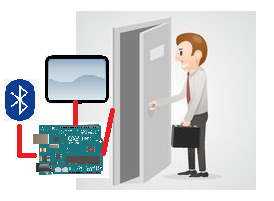
\includegraphics[width = 300 pt]{Img/Konceptbillede.png}
	\caption{Konceptbillede}
	\label{fig:Konceptbillede}
\end{figure}

	%!TEX root = ../../Main.tex
\graphicspath{{Chapters/Krav/}}
%-------------------------------------------------------------------------------


\section{Krav}
I dette afsnit beskrives kravene til hvilken funktionalitet systemet har. 


I samarbejde med vejleder er der opstillet en række krav.
\begin{itemize}
\item Systemet skal kunne finde de 4 stærkeste bluetooth signaler. 
\item Systemet skal kunne køre "hele tiden"
\item Systemet skal opdateres en gang i hvert sekund.  
\end{itemize}


%!TEX root = ../../Main.tex
\graphicspath{{Chapters/System/}}
%-------------------------------------------------------------------------------


\section{System beskrivelse}

BA-TA's (Bluetooth Anti-Theft Alarm) primære funktionalitet ligger i hhv. at kunne låse op og låse hoveddøren, så snart systemet registrerer at husets ejer (og dermed smartphone) eller en anden godkendt Bluetooth-enhed, er i nærheden eller ej.

Igennem brugergrænsefladen kan brugeren både tilføje og fjerne de godkendte Bluetooth-enheder (personer) som skal kunne låse og låse op for døren.

Når alle godkendte enheder er uden for rækkevidde af systemets Bluetooth-modul, låses døren, og så snart systemet ser en godkendt enhed indenfor rækkevidden bliver døren igen låst op. 

I under-afsnittende herunder bliver systemets blokke og de interne fobindelser præsenteret.
På figur \ref{fig:Bdd} ses et overordnet Bdd for projektet, hvor de interne forbindelser forklares på figur \ref{fig:Ibd}. 

\begin{figure}[H]
	\centering
	\includegraphics[width = 500 pt]{Img/Bdd.png}
	\caption{Bdd af BA-TA}
	\label{fig:Bdd}
\end{figure}

\subsection{Blokbeskrivelse BA-TA}
\textbf{Arduino} \\*
Arduino'en, mega2560, initialiserer og styrer alt funktionaliteten som indgår i systemet. Arduino blokken står for at initialisere  Touch Display, Touch Controller og Display Controller som bruges til at kunne modtage signaler fra Touch-delen, samt at sende signaler til Display'et og dermed få repræsenteret noget til brugeren. Yderligere bruges Arduinoen til at initialisere og kontrollere UART driveren og Bluetooth modulet.
\newline
\newline
\textbf{Touch Controller} \\*
Touch Controller står for at modtage værdier fra Touch Display, samt at sende den modtagede værdi videre til Arduino'en. 
\newline
\newline
\textbf{Display Controller} \\*
Display Controller modtager værdier fra Arduino'en og sende sende værdien videre til Touch Display. \newline
\newline
\textbf{Bluetooth} \\*
Bluetooth modul, HC-05, som kommunikkerer med Arduino'en vha. AT-kommandoer.
\newline
\newline
\textbf{Touch Display} \\*
Touch Display fungerer som brugergrænseflade og er dermed måden brugeren kan interagere med systemet. 
\newline
\newline
\textbf{Lock} \\*
Lock er den fysiske lås, denne er ikke implementeret i projektet, men simuleres med en visuel lås på skærmen. 
\subsection{Internal Block Diagram for BA-TA}
På figur \ref{fig:Ibd} ses et overordnet IBD over selve systemet, som er bygget på Bdd'et. 
\begin{figure}[H]
	\centering
	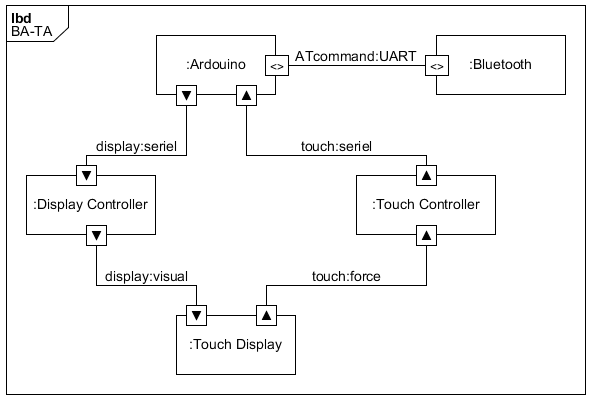
\includegraphics[width = 300 pt]{Img/Ibd.png}
	\caption{Ibd af BA-TA}
	\label{fig:Ibd}
\end{figure}




	%!TEX root = ../../Main.tex
\graphicspath{{Chapters/Userinterface/}}
%-------------------------------------------------------------------------------


\section{Brugergrænseflade}
I dette afsnit gives der et overblik over brugergrænsefladen og brugerens mulighed for interaktion med denne. Afsnittet er bygget op af billeder, hvor hvert billede viser brugergrænsefladens visuelle struktur. \\

Første display man møder er "Welcome". Her går systemet igang med at initialisere de forskellige moduler og drivere, således de er klar til brug.
\begin{figure}[H]
	\centering
	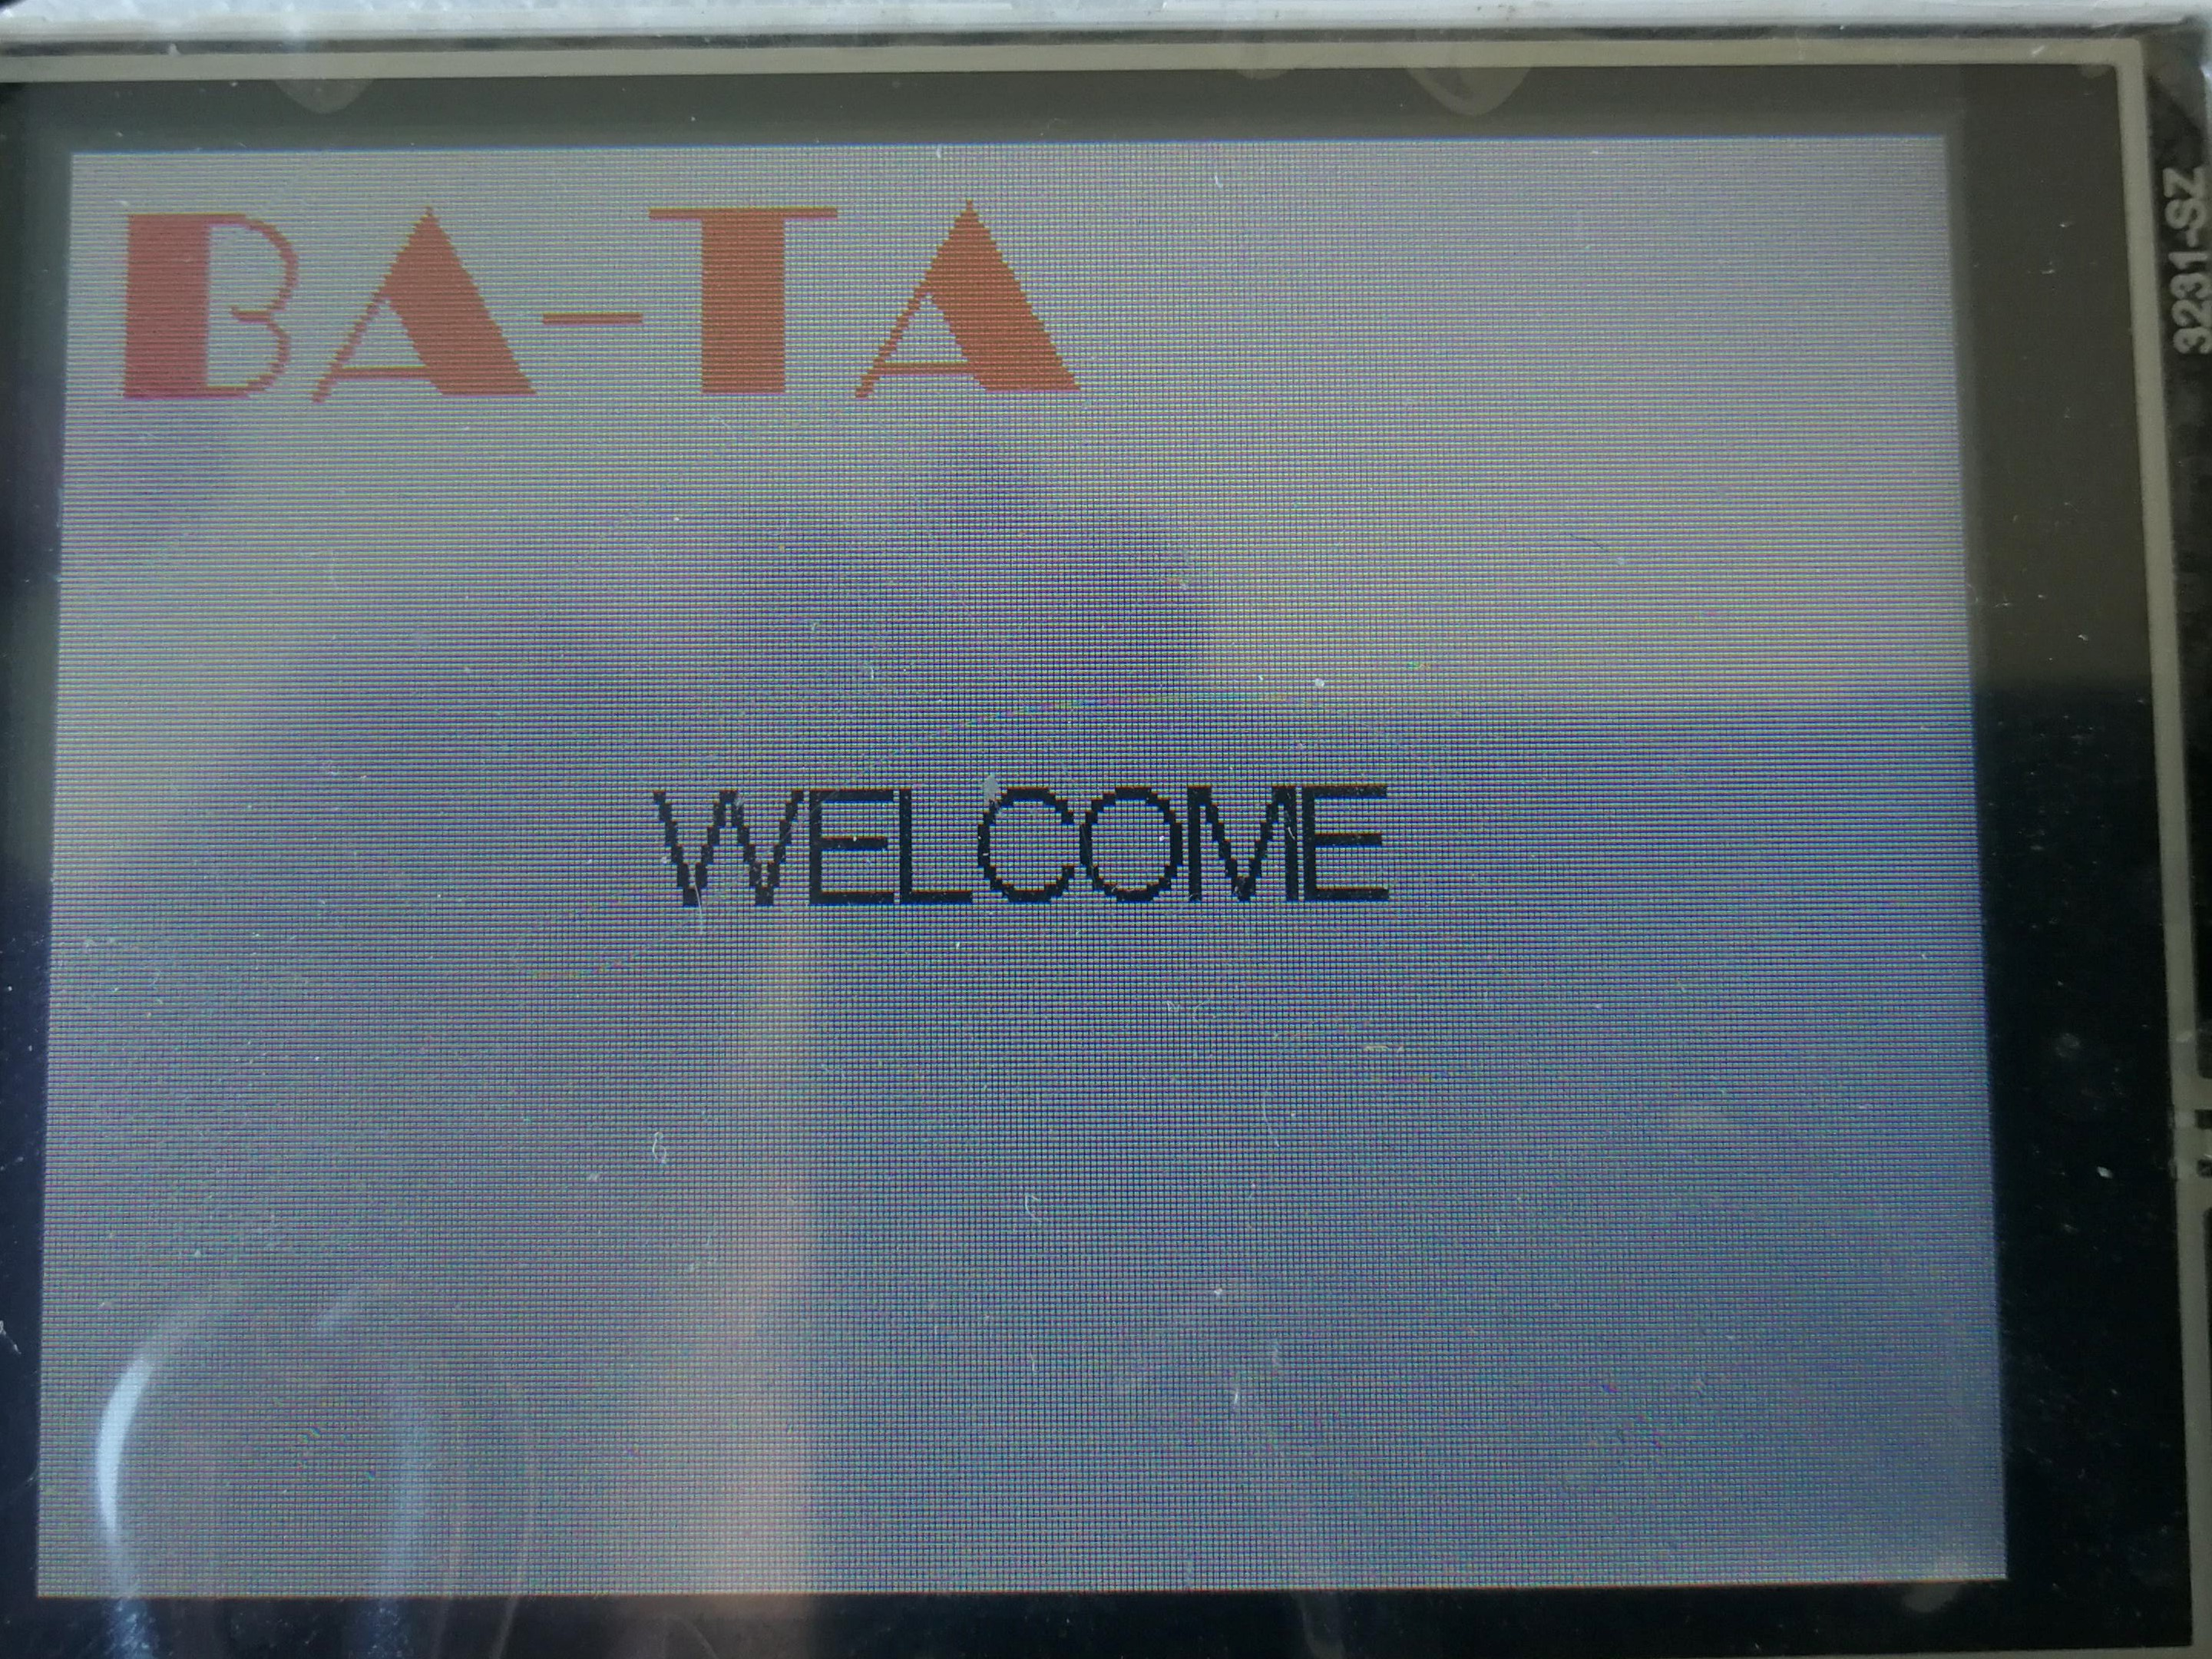
\includegraphics[width = 300 pt]{Img/welcome.jpg}
	\caption{Brugergrænseflade: Welcome}
	\label{fig:welcome}
\end{figure}

Næste display er hovedmenuen for systemet, hvor der er tre forskellige muligheder, som ses på figur     \ref{fig:start}. Yderligere ses der 4 trykknapper, hvor brugeren kan interagere med systemet.

\begin{itemize}  
	\item  Med "Enter" vælger brugeren en funktion
	\item "Back" gør brugeren i stand til at gå tilbage til hovedmenuen, hvis man forinden har trykket "ENTER" ved "ADD DEVICE" eller "REMOVE DEVICE".
	\item "Up" og "Down" flytter pilen, hhv. op og ned.
\end{itemize}

 Herudover ses der en farvet boks øverst i højre hjørne, som indikerer låsens tilstand. Denne lås viser grøn ved låst op og rød ved låst. Øverst til venstre på skærmen vises systemets logo.    
\begin{figure}[H]
	\centering
	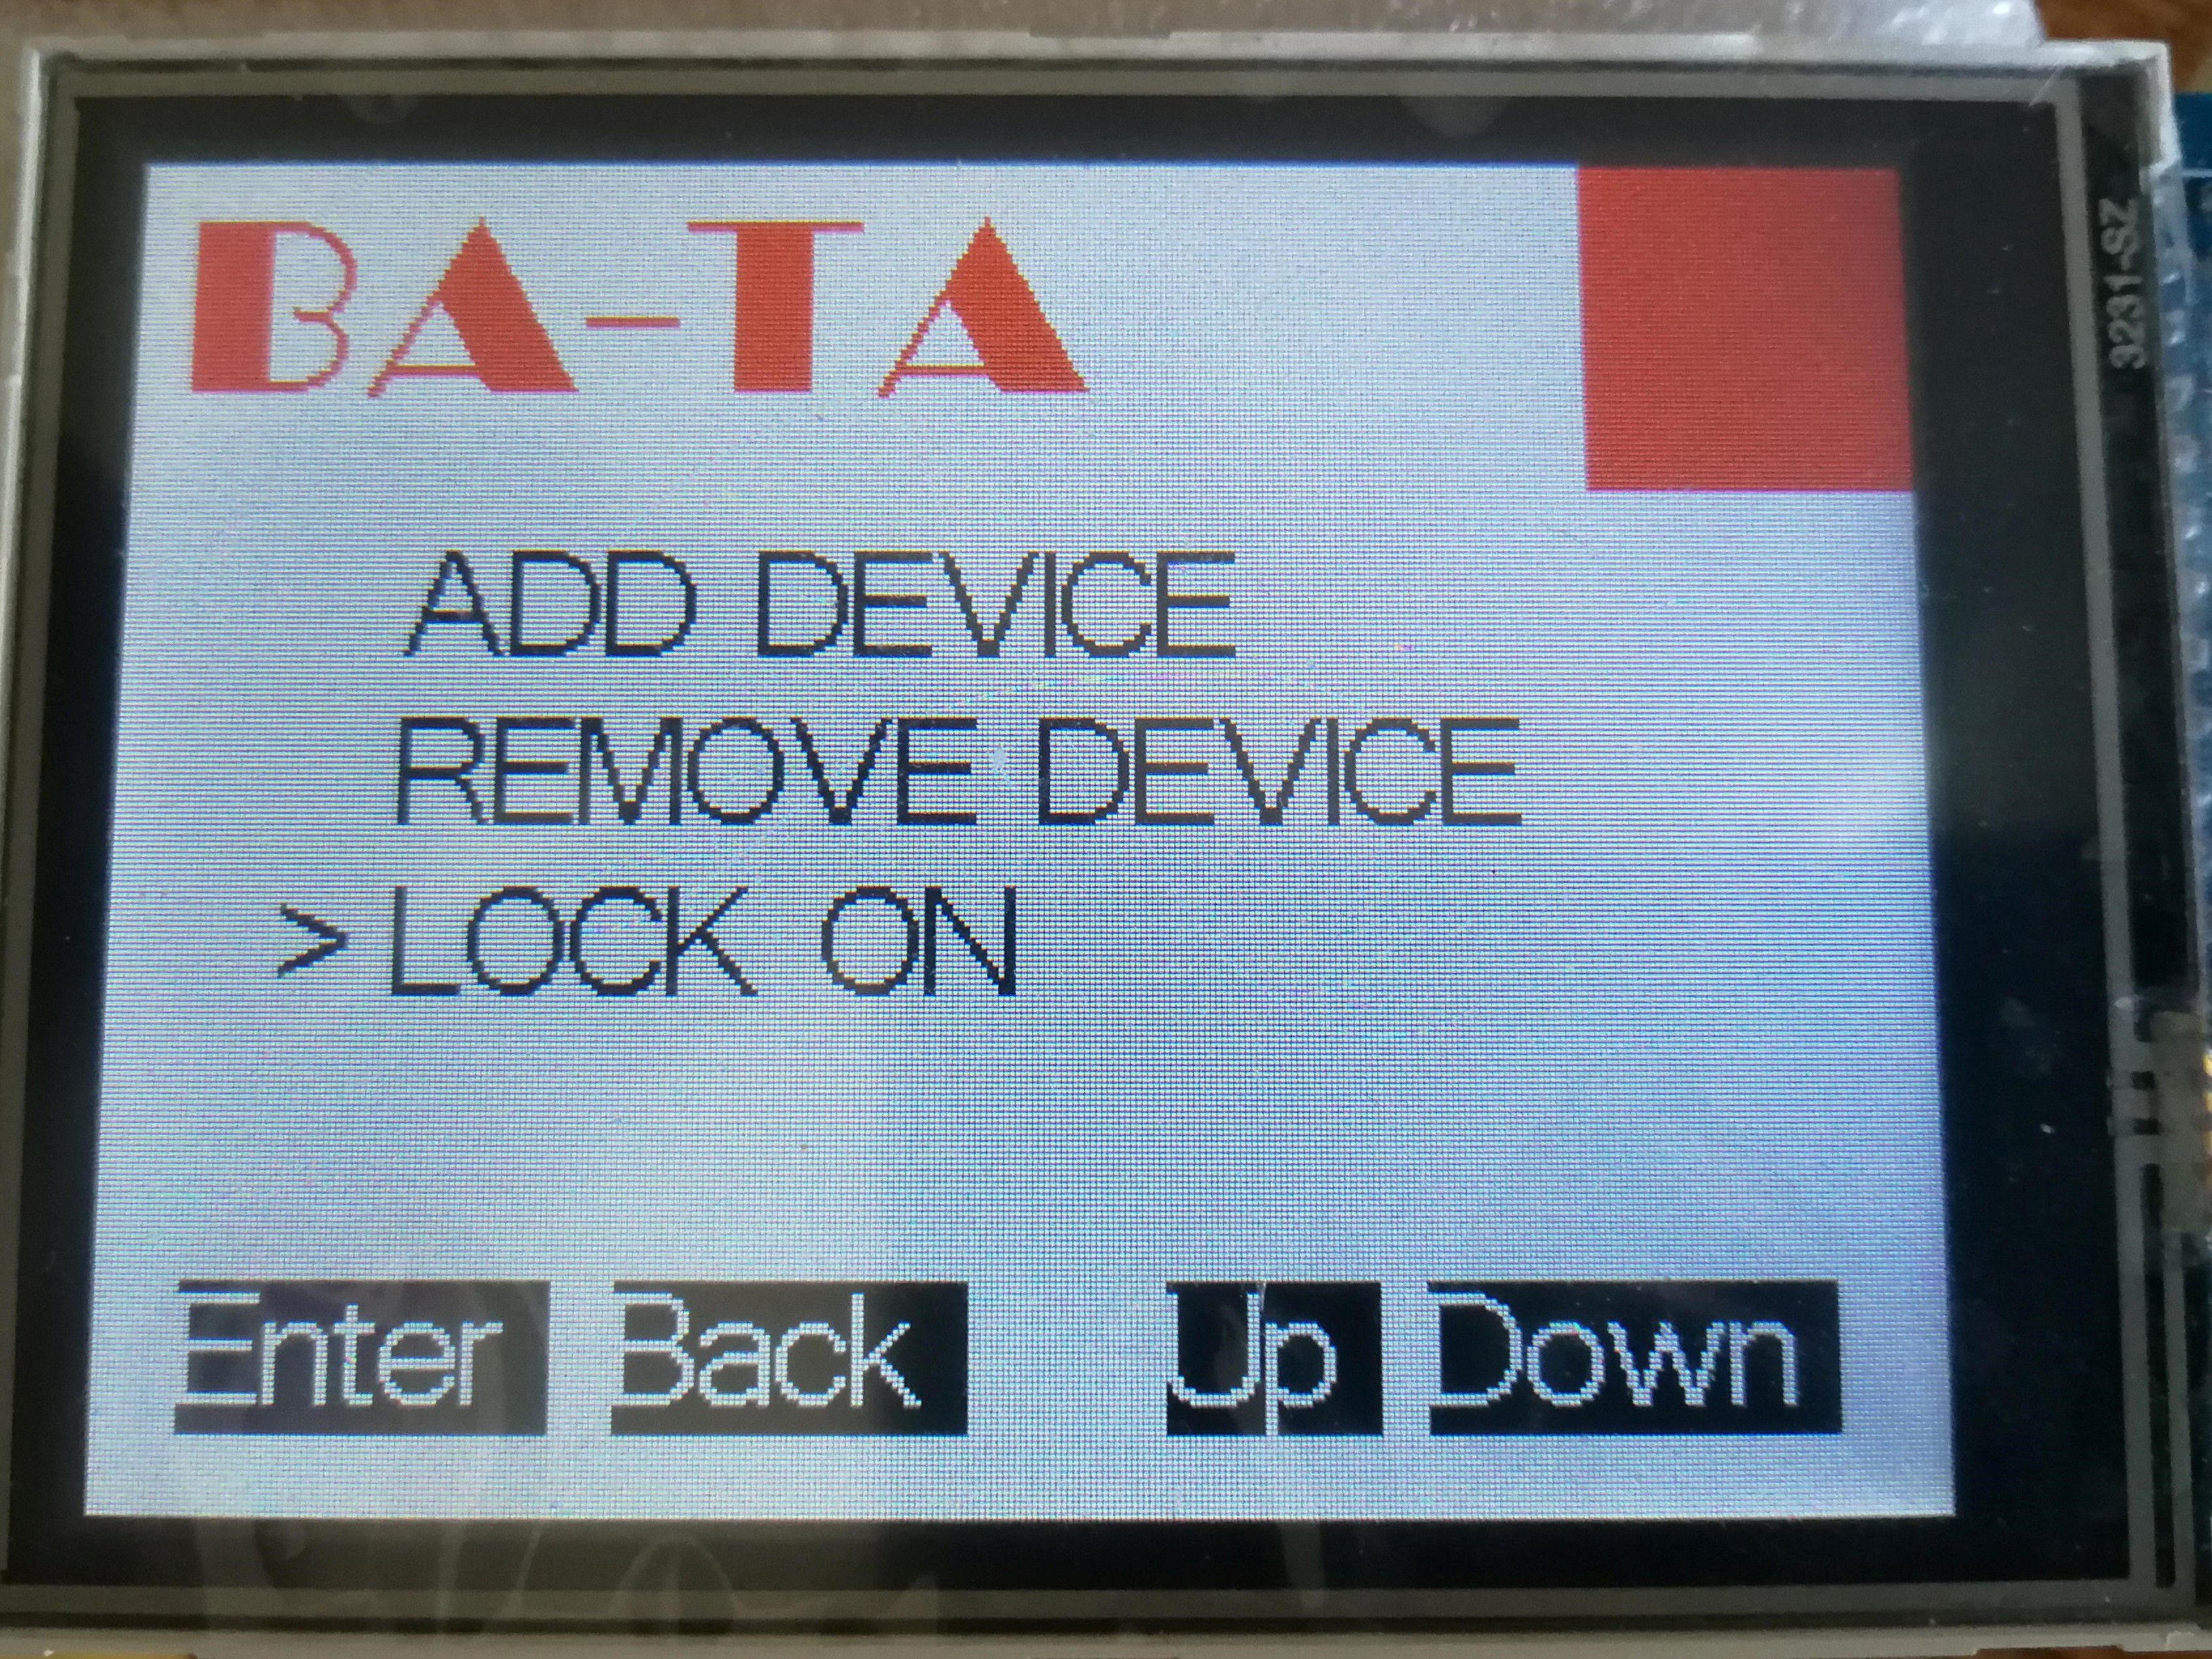
\includegraphics[width = 300 pt]{Img/start.jpg}
	\caption{Brugergrænseflade: Hovedmenu}
	\label{fig:start}
\end{figure}

Hvis brugeren trykker på "ADD DEVICE", søger BA-TA efter de 4 stærkeste Bluetooth signaler, som er indenfor rækkevidde. 
\begin{figure}[H]
	\centering
	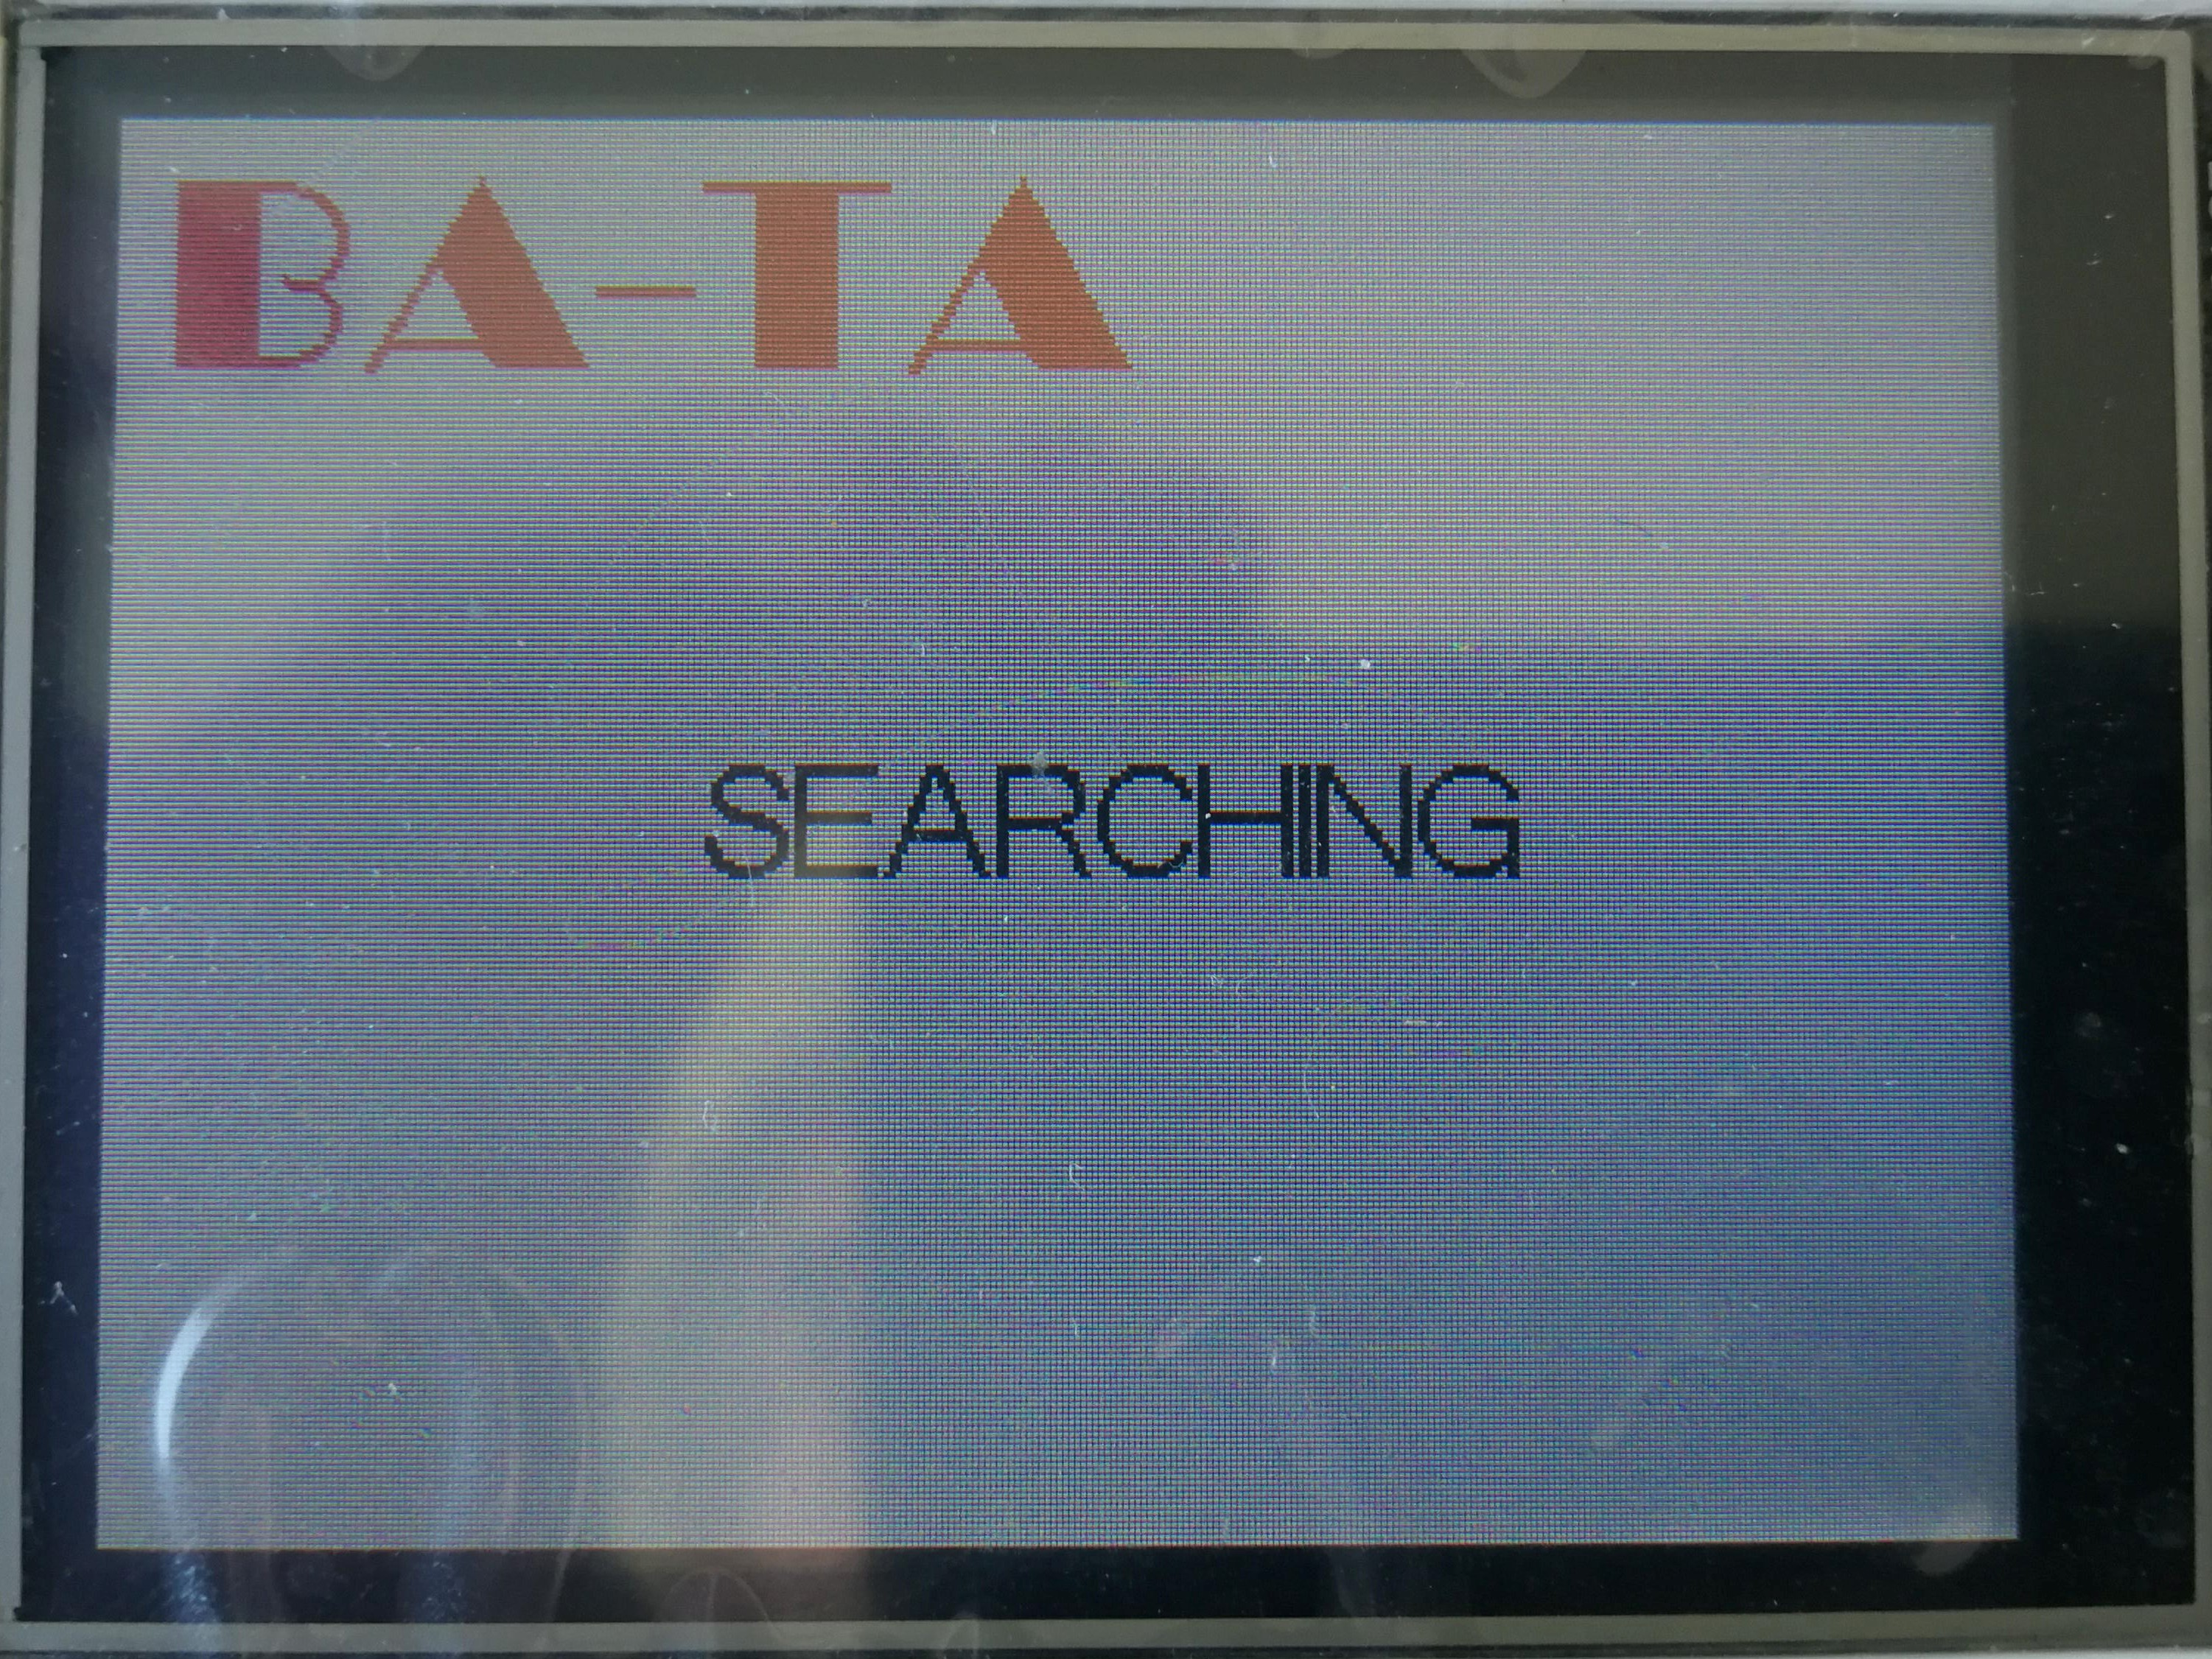
\includegraphics[width = 300 pt]{Img/Searching.jpg}
	\caption{Brugergrænseflade: Searching}
	\label{fig:Searching}
\end{figure}
Herefter vises de fundne Bluetooth-enheder, som systemets Bluetooth-modul har fundet. Dette ses på figur \ref{fig:devices}.
\begin{figure}[H]
	\centering
	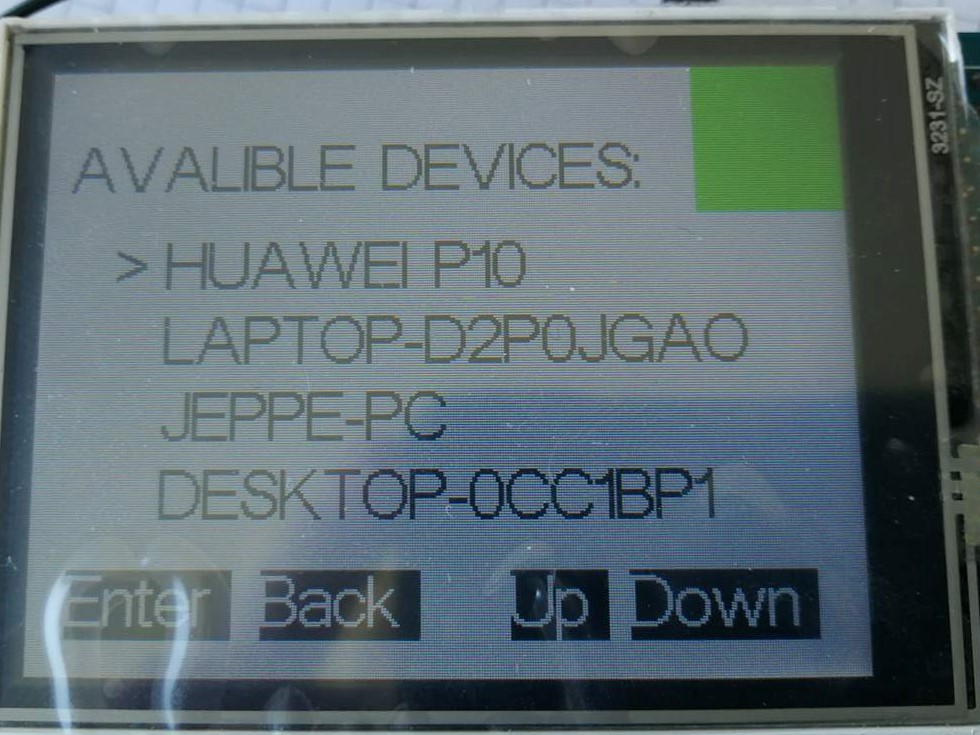
\includegraphics[width = 300 pt]{Img/devices.jpg}
	\caption{Brugergrænseflade: Tilgængelige enheder}
	\label{fig:devices}
\end{figure}
Hvis der vælges en enhed ved et tryk på "Enter", så vises navnet på den valgte enhed. Herefter går skærmens tilstand tilbage til hovedmenuen. 
\begin{figure}[H]
	\centering
	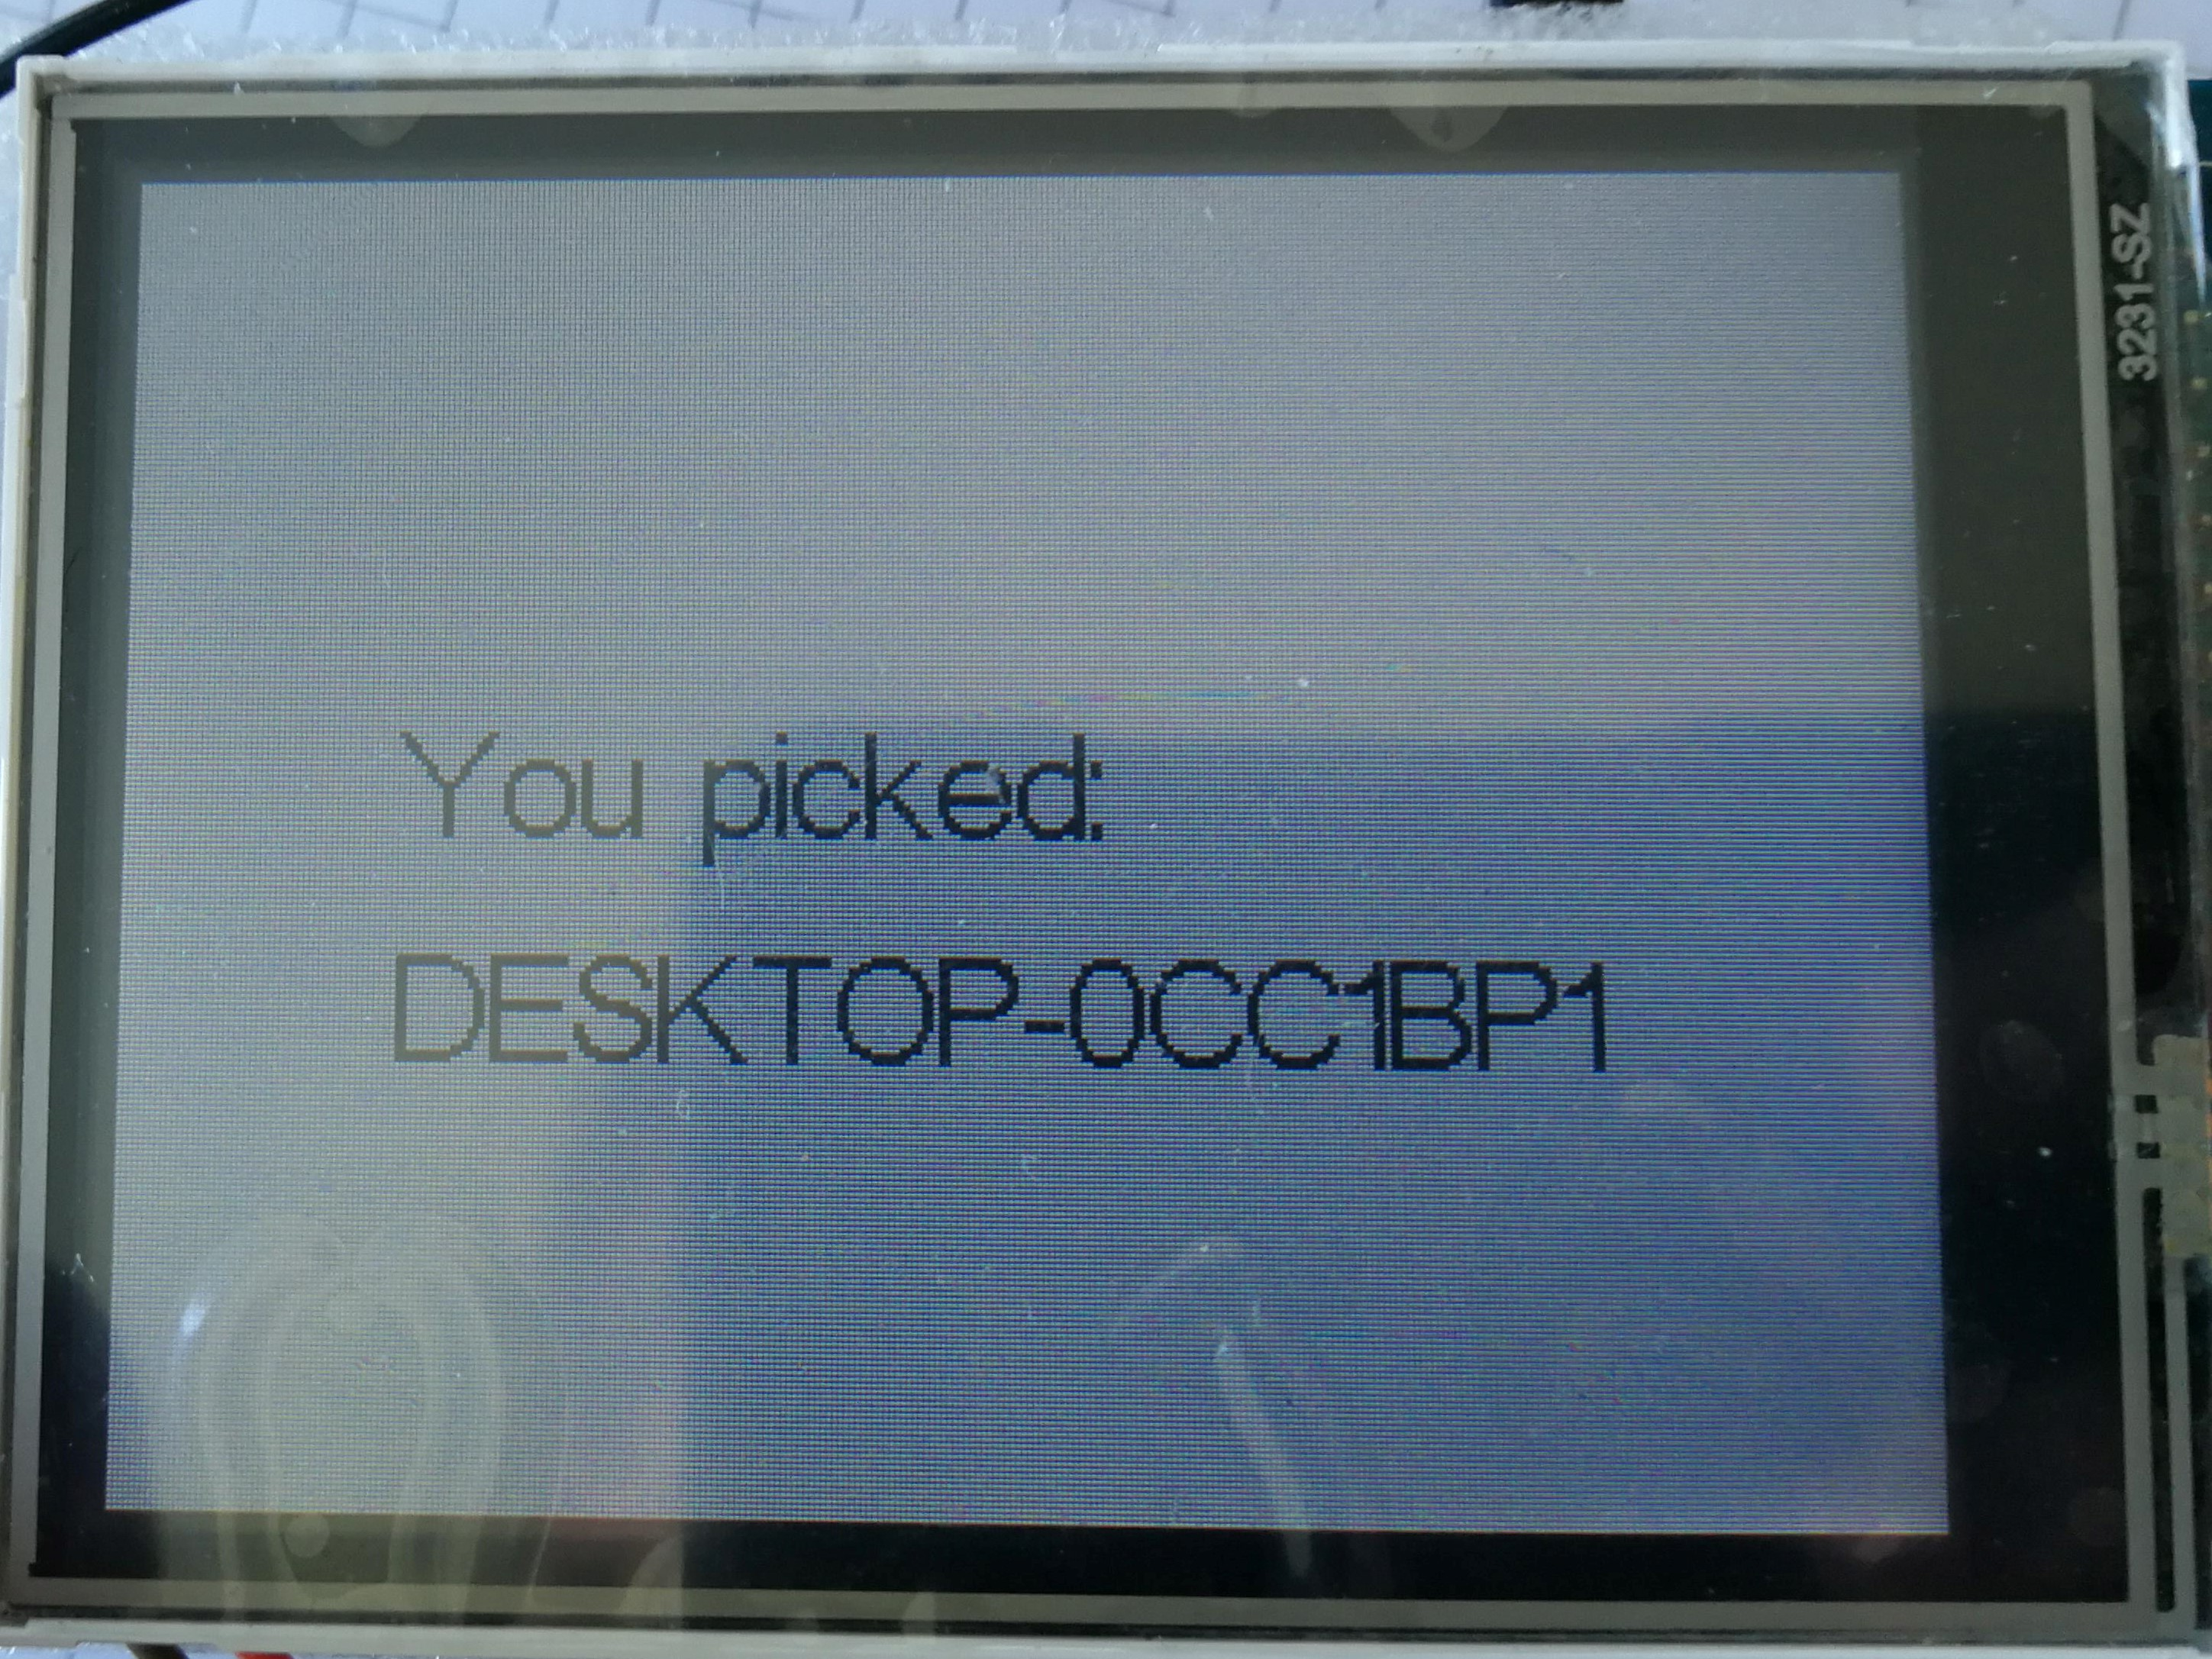
\includegraphics[width = 300 pt]{Img/pick.jpg}
	\caption{Brugergrænseflade: Valg af enhed}
	\label{fig:pick}
\end{figure}
Hvis brugeren herefter vælger funktionen "REMOVE DEVICE" fra figur \ref{fig:start}, åbnes der en liste over de godkendte Bluetooth-enheder der er gemt. Dette ses på figur \ref{fig:remove}. Hvis der på forhånd ikke er nogle gemte godkendte Bluetooth-enheder og listen dermed er tom, så vil displayet også være tomt, som vist på figur \ref{fig:noDevices}. 
\begin{figure}[H]
	\centering
	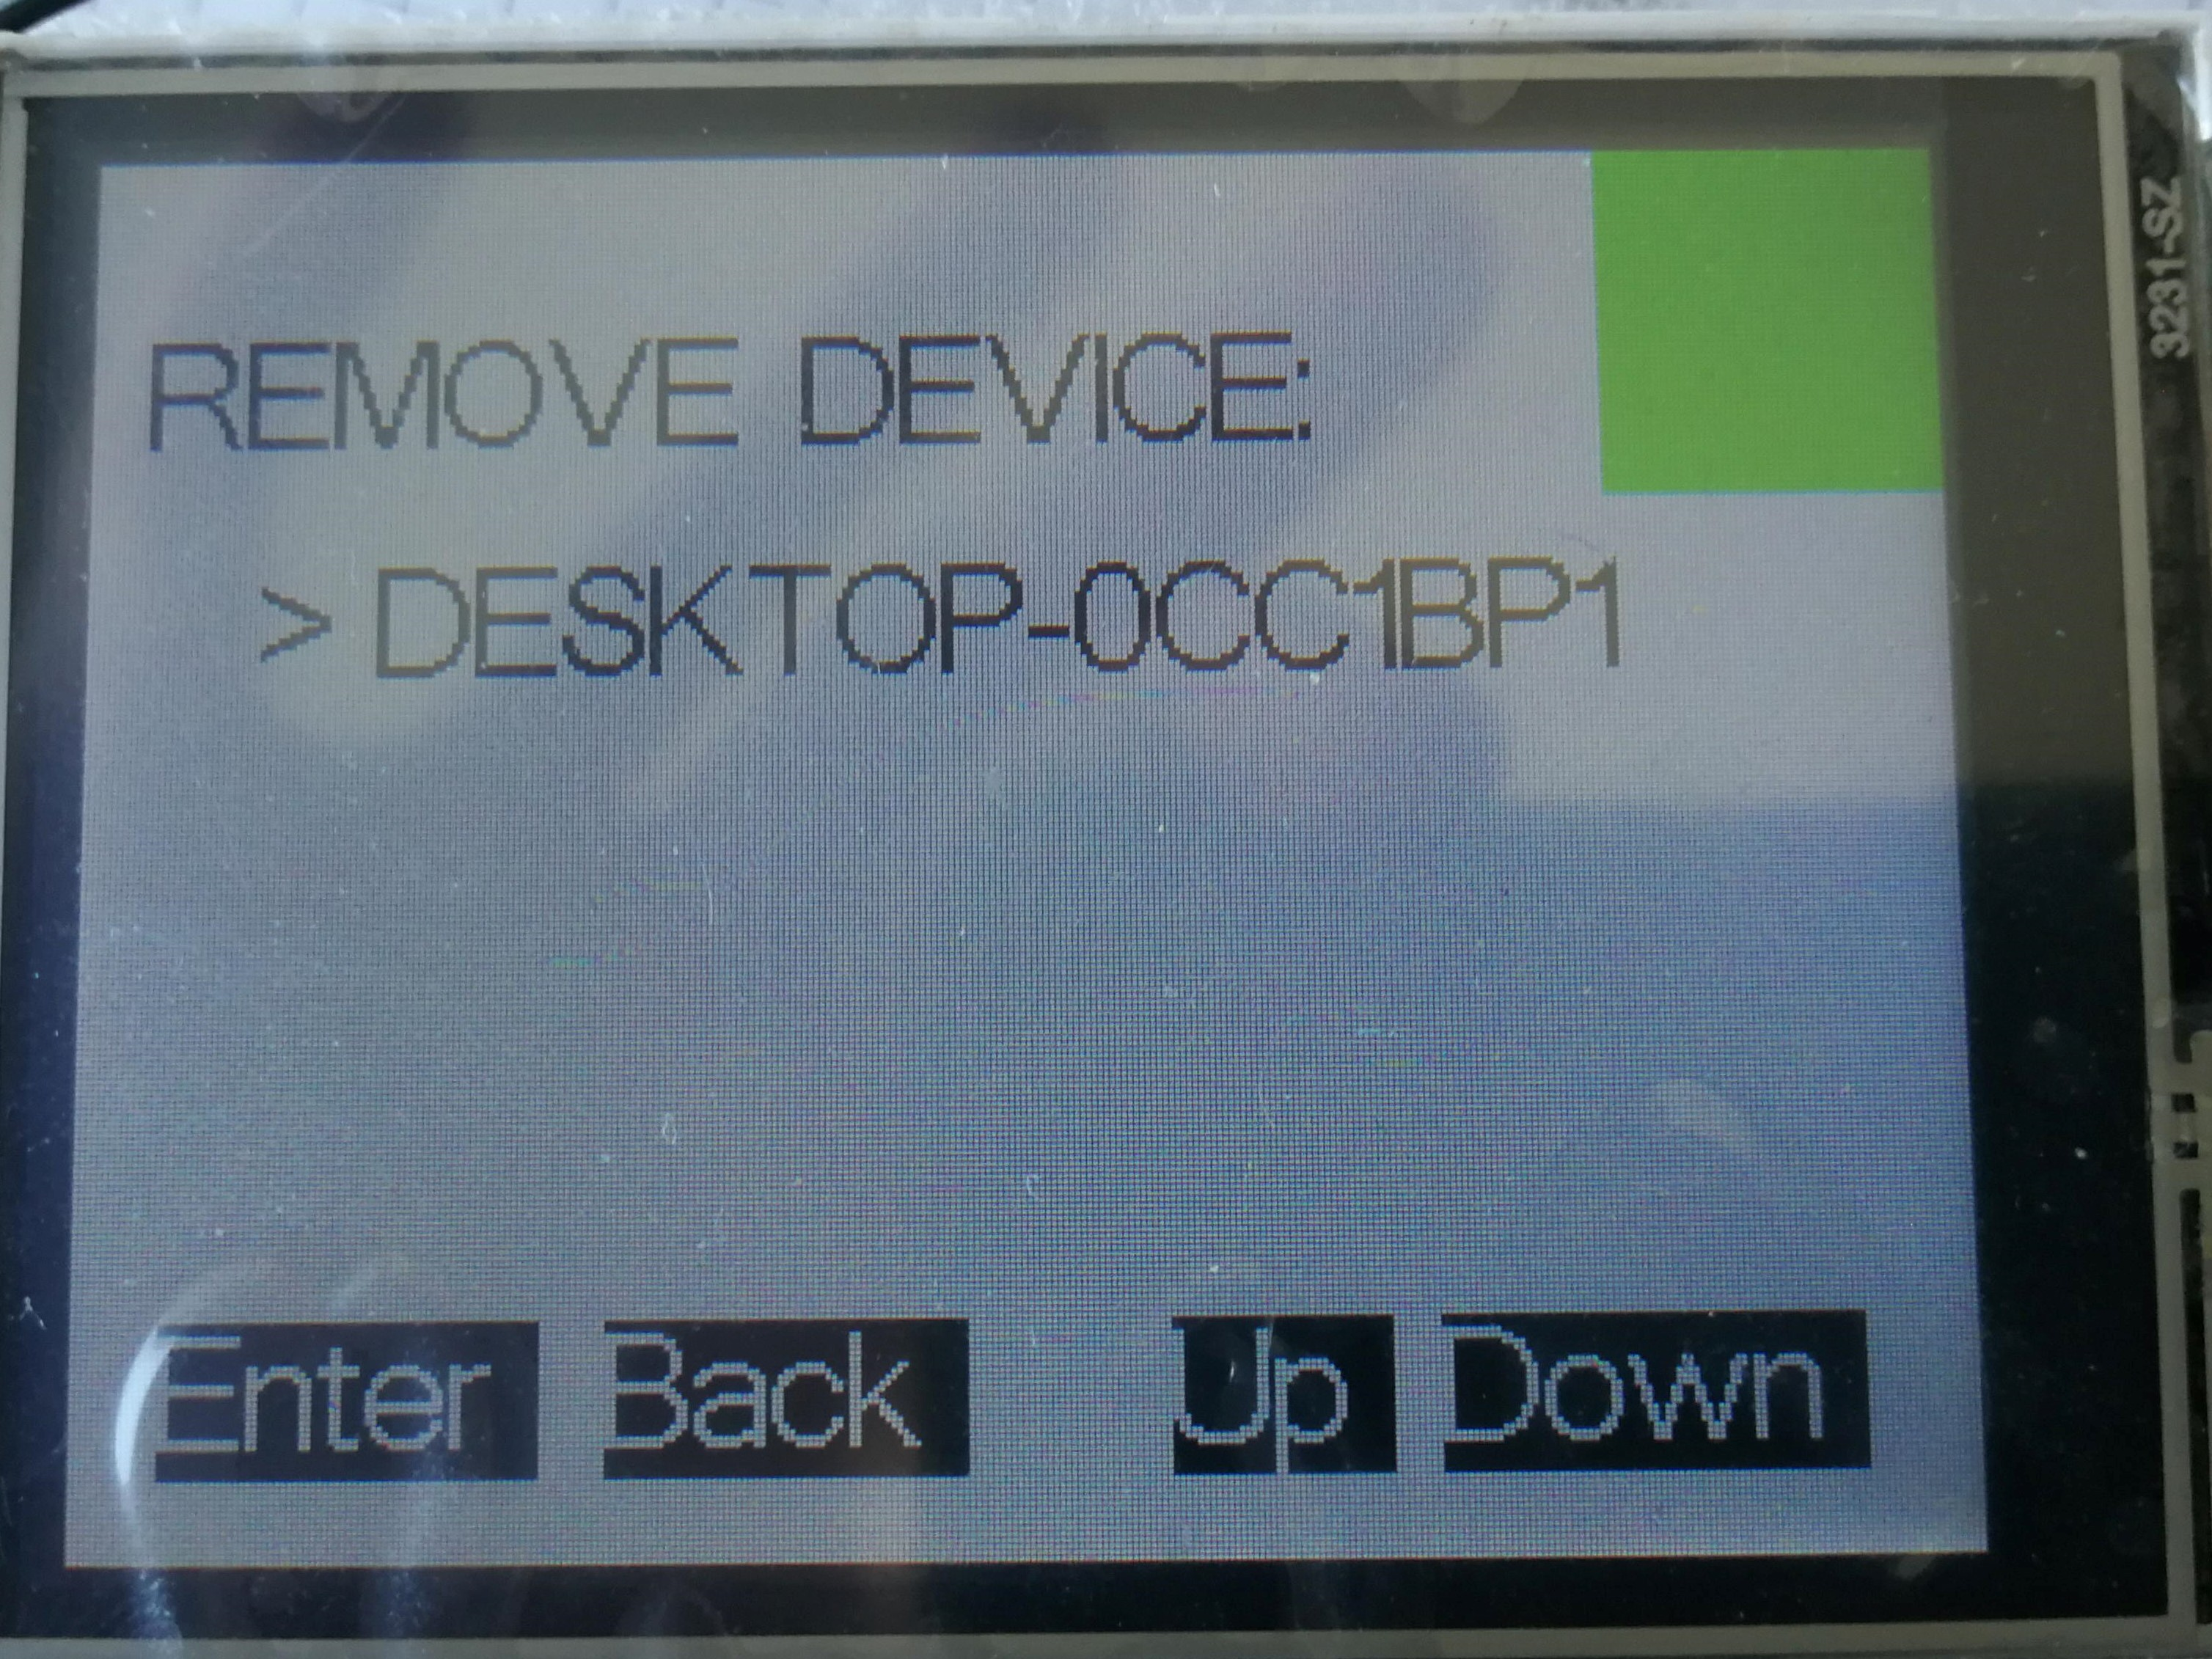
\includegraphics[width = 300 pt]{Img/remove.jpg}
	\caption{Brugergrænseflade: Fjern en enhed}
	\label{fig:remove}
\end{figure}
\begin{figure}[H]
	\centering
	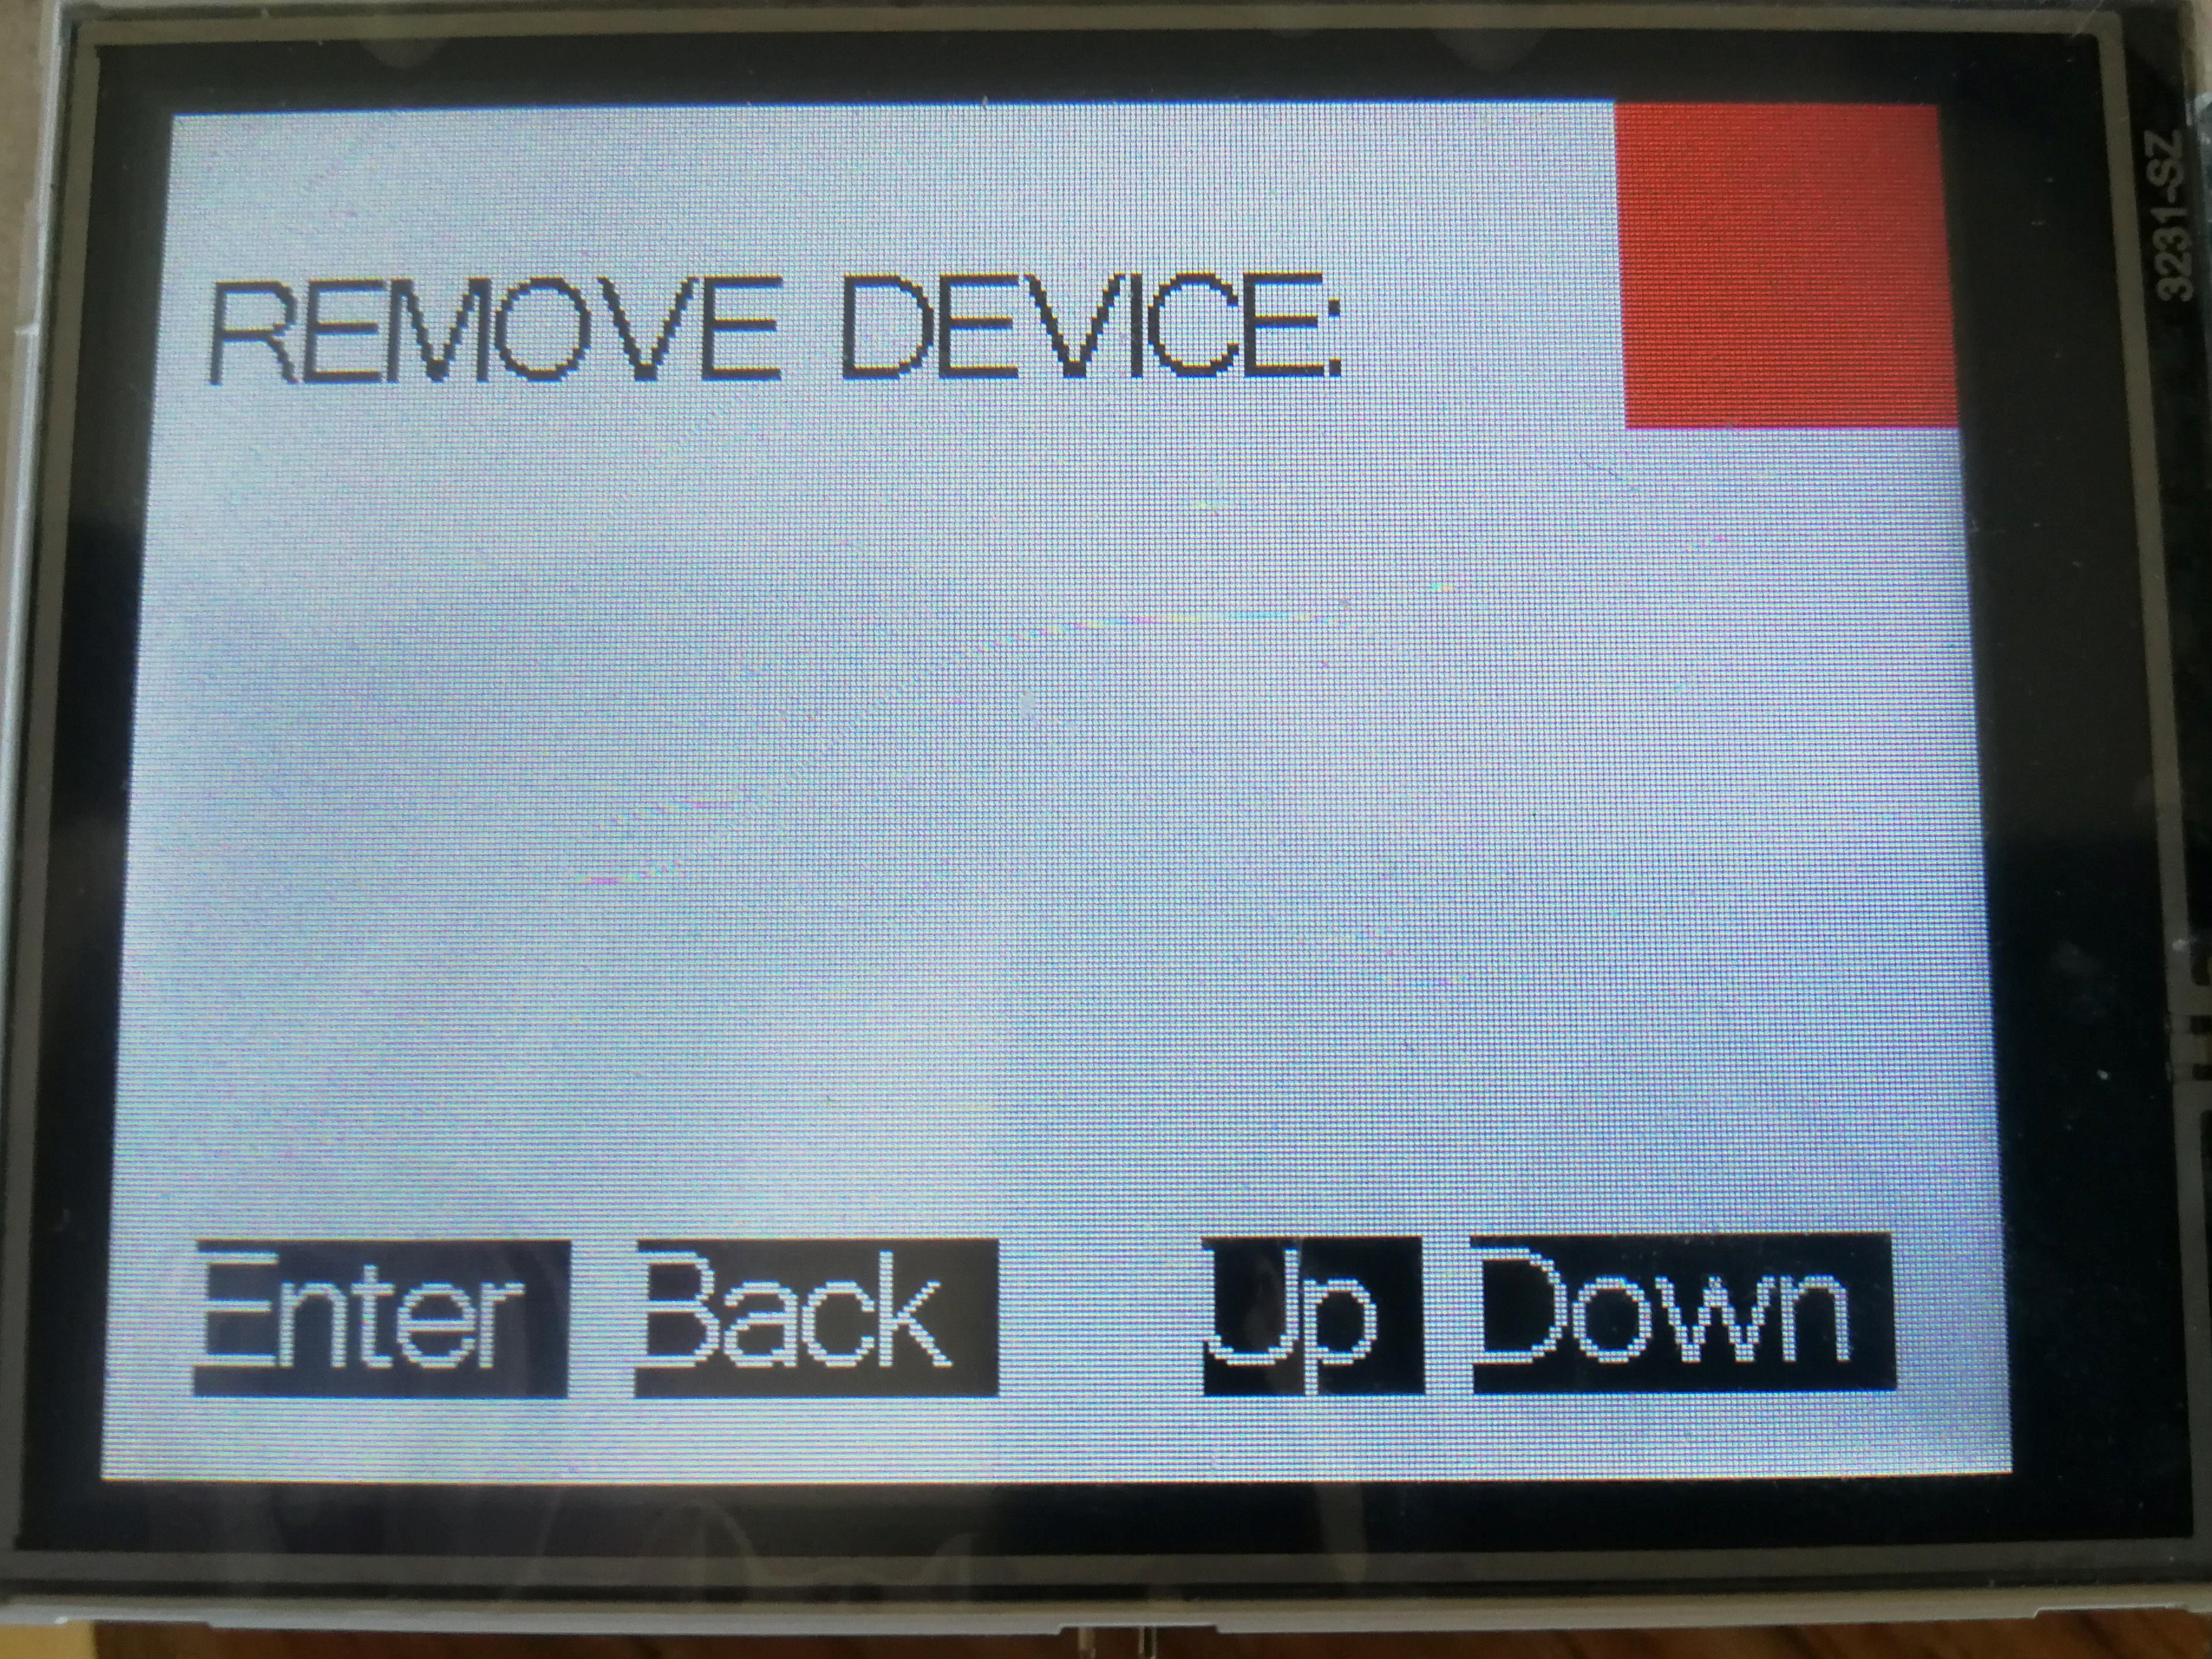
\includegraphics[width = 300 pt]{Img/noDevice.jpg}
	\caption{Brugergrænseflade: Ingen enehder}
	\label{fig:noDevices}
\end{figure}
Såfremt der er godkendte Bluetooth-enheder på listen, kan brugeren vælge at slette en bestemt enhed. Dette sker ved at trykke "Enter" ved enheden, som vælges ved hjælp af "Up" og "Down" og indikeres af pilen. Displayet viser på figur \ref{fig:delete} en besked om hvilken enhed brugeren har valgt at slette. 
\begin{figure}[H]
	\centering
	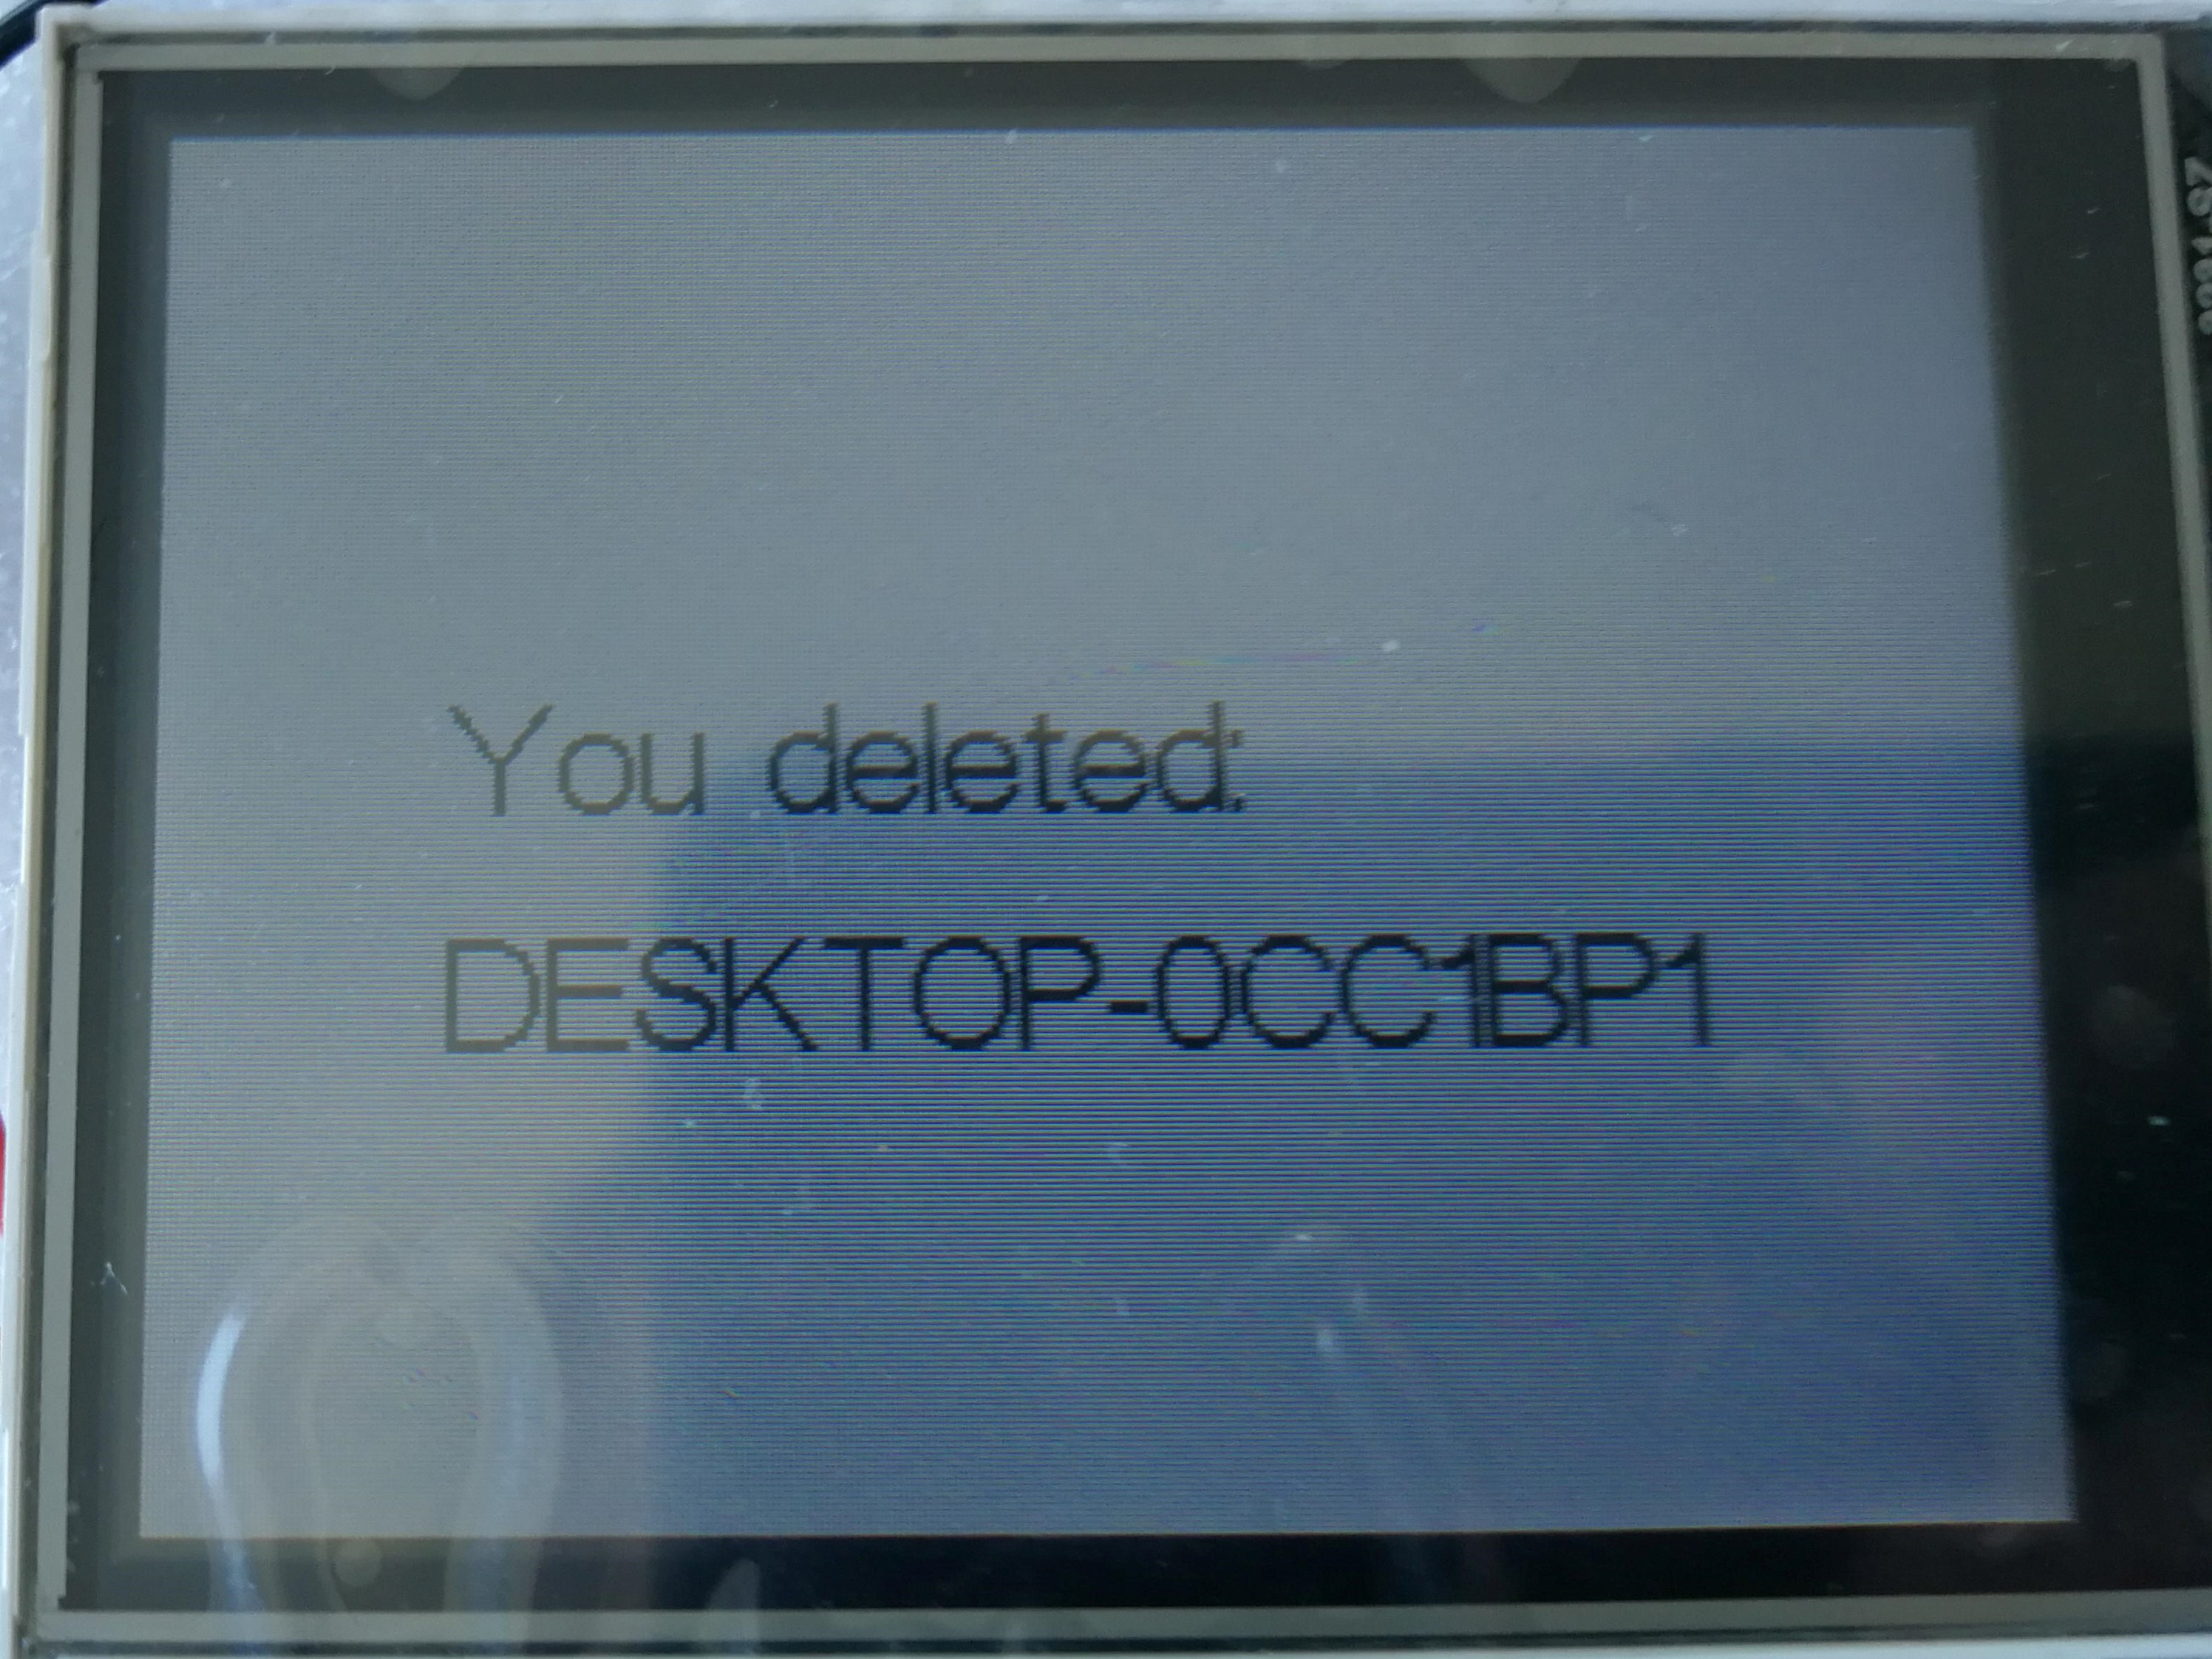
\includegraphics[width = 300 pt]{Img/delete.jpg}
	\caption{Brugergrænseflade: Valgt: fjernet en enhed}
	\label{fig:delete}
\end{figure}
Hvis brugeren vælger den sidste mulighed/state i hovedmenuen, "LOCK OFF", låses systemet op, teksten skifter og låsens indikator skifter farve. Dette ses på \ref{fig:lockOff}.
\begin{figure}[H]
	\centering
	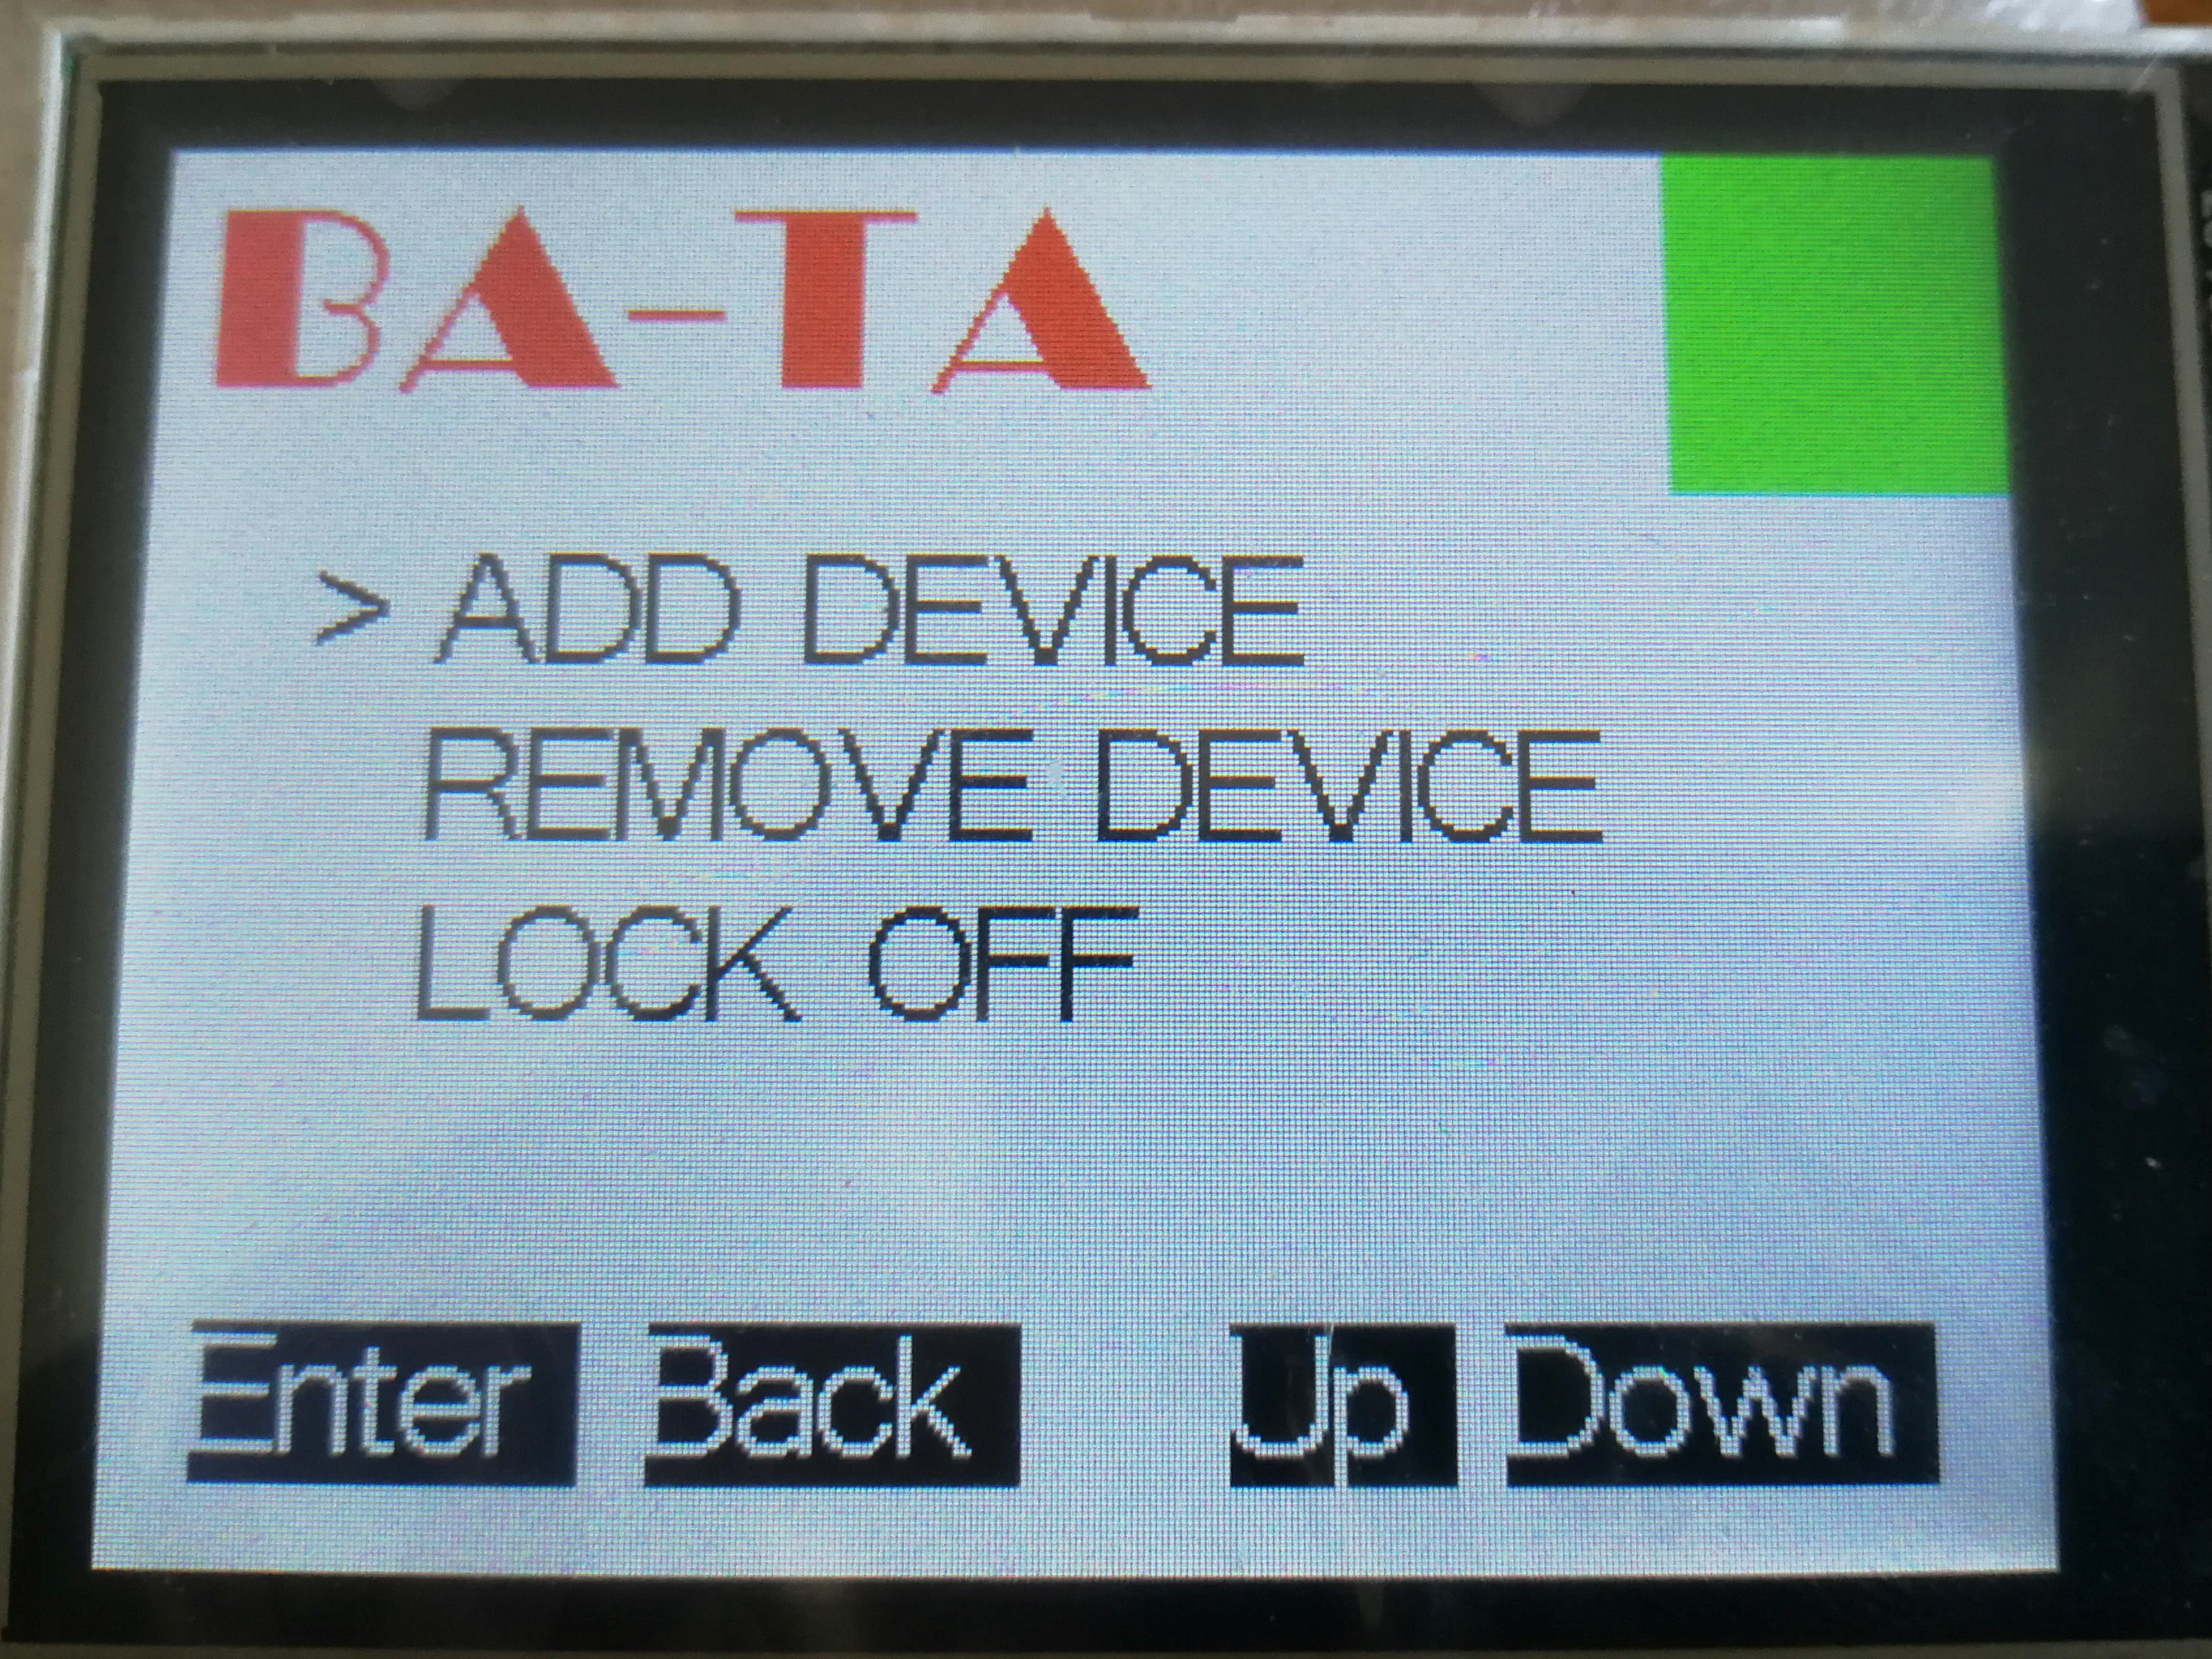
\includegraphics[width = 300 pt]{Img/lockOff.jpg}
	\caption{Brugergrænseflade: Låst op}
	\label{fig:lockOff}
\end{figure}
Hvis der endnu engang trykkes på den sidste state i hovedmenuen, ændres teksten, og låsen laver en "UPDATE"  hvert 5. sekund, og skifter låsen alt efter om der kan findes en Bluetooth-enhed, som også er på den godkendte liste. Dette ses på figur \ref{fig:auto}. Hvis der trykkes én gang til på sidste state, ændres låsens tilstand til at være manuelt låst.
\begin{figure}[H]
	\centering
	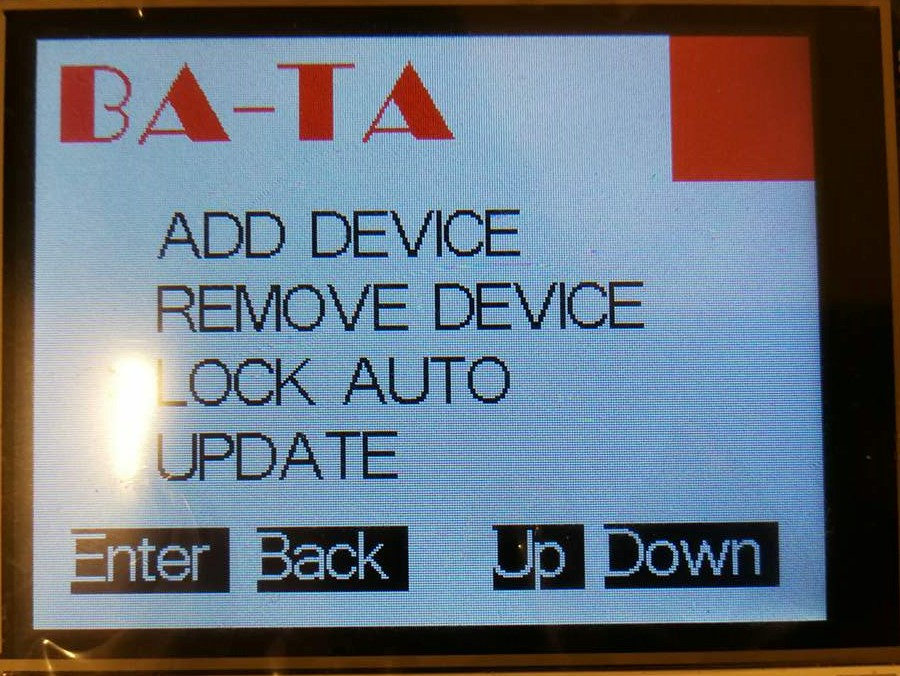
\includegraphics[width = 300 pt]{Img/auto.jpg}
	\caption{Brugergrænseflade: Lås Automatisk}
	\label{fig:auto}
\end{figure}


%!TEX root = ../../Main.tex
\graphicspath{{Chapters/Struktur/}}
%-------------------------------------------------------------------------------

\section{Graphic display driver}

Som brugergrænseflade i dette projekt bruges et ITDB02, som er valgt da der tidligere er arbejdet med netop dette produkt. Dertil kommer ILI9341 som driver til selve display'et. 

Driver softwaren til hele displayet, er delt op i flere forskellige cpp filer, dette er gjort for at gøre koden mere overskuelig, og gøre funktionaliteten mere effektiv. Herunder forsøges at gøre et overblik over de forskellige cpp filer og deres integeren. 


\begin{figure}[H]
	\centering
	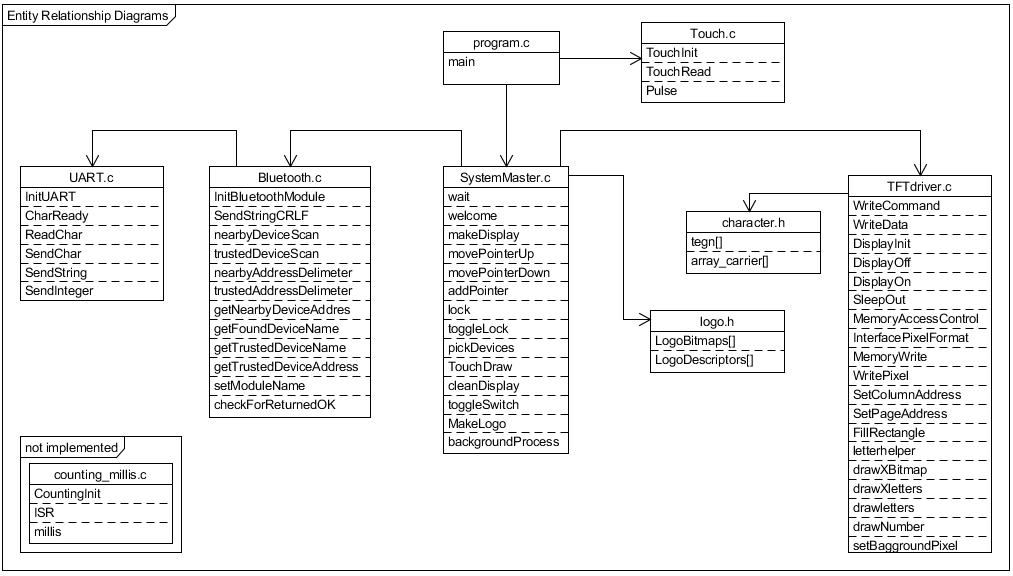
\includegraphics[width = 300 pt]{Img/Entity.png}
	\caption{Entity Relationship Diagrams}
	\label{fig:Konceptbillede}
\end{figure}
 
---Skriv noget når det hele er færdig her




%!TEX root = ../../Main.tex
\graphicspath{{Chapters/Display/}}
%-------------------------------------------------------------------------------


\section{Display driver}
Igennem øvelser til undervisningen, er der blevet opbygget en driver til et grafisk display. Igennem processen til dette projekt er der blevet modificeret og arbejdet videre på selvsamme driver. Cpp filen ligger under TFTdriver, som er bygget op af flere forskellige funktioner. I dette afsnit vil der gives et overblik over de mest essentielle funktioner. For at få en forståelse af selve opbygningen af driveren, henvises til datasheet for controlleren. 
\href{https://blackboard.au.dk/bbcswebdav/pid-1697983-dt-content-rid-3847230_1/courses/BB-Cou-UUVA-73302/BB-Cou-UUVA-65758_ImportedContent_20170106021228/BB-Cou-STADS-UUVA-52360_ImportedContent_20160107025559/LAB/Lab3a%20Graphic%20LCD%20Display/Files%20for%20LAB3a/ILI9341_v1.11.pdf}{ILI9341} \\
For at opbygge en basisforståelse for driveren, vil der først blive forklaret DisplayInit(). Først sætter vi de porte vi skal bruge fra Arduino til hhv. indgange og udgange. Vi har dog valgt ikke at have tilbagemeldinger, og derfor er der ikke initialiseret nogle indgange. Herefter sætter vi RESET, CS, WRX, RDX høje ift figur \ref{fig:Bus_timing}. Der bliver kørt en reset (tjek lige koden med timing, burde være kortere), for at resette displayet, og bagefter sendt fire kommandoer, som kan findes i command list i databladet. Sleep Out, Display On, Pixel format set = 16 bit og Memory Access Control (BGR = 1) (Tjek ift henning hvad dette gør). 



\begin{figure}[H]
	\centering
	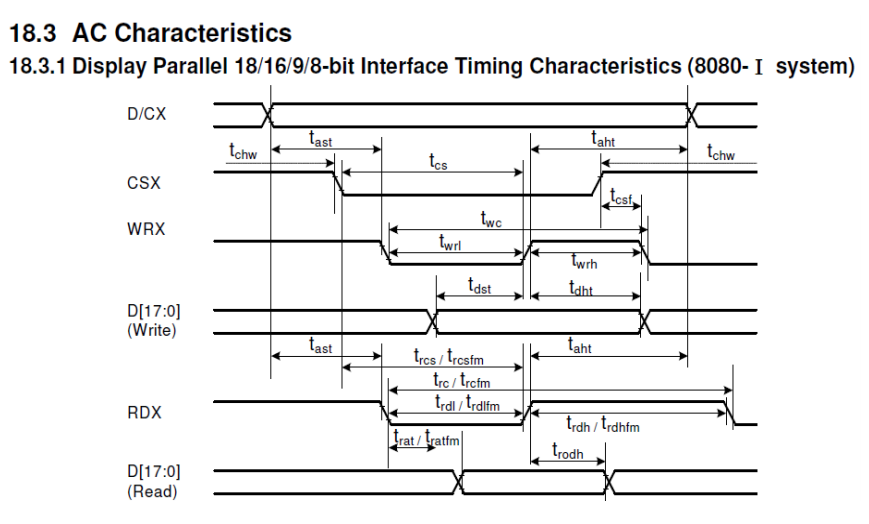
\includegraphics[width = 400 pt]{Img/Bus_timing.png}
	\caption{Bus Timing}
	\label{fig:Bus_timing}
\end{figure}

Herunder vil de essentielle funktioner deles op i hvert sin tabel. Flere af funktionerne gør brug af både Writecommand() og Writedata(), som er opbygget udfra Bus Timing figur \ref{fig:Bus_timing}. Derudover bruger flere af funktionerne SetColumnAddress() og SetPageAddress(), som er bygget op fra datasheet 8.2.20. og 8.2.21.: \\

\newpage
\textbf{\Large Included Font:}

\begin{center}
\begin{tabular}{ |l|l|l| }
\hline
\multicolumn{1}{ |c| }{\textbf{character.h}} \\
\hline
Karakter størrelse: 24*24 pixels  \\
Antal karakter: 95\\
\hline

\end{tabular}
\end{center} 
\begin{figure}[H]
	\centering
	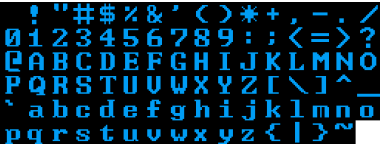
\includegraphics[width = 150 pt]{Img/Thedotfactory.png}
	\caption{The Dot Factory karakter}
	\label{fig:Thedotfactory}
\end{figure}

\textbf{\Large Funktions:}

\begin{center}
\begin{tabular}{ |l|l|l| }
\hline
\multicolumn{1}{ |c| }{\textbf{ FillRectangle(StartX,StartY, Width, Height, Red, Green, Blue)}} \\
\hline
Funktion som laver en firkant med den valgte baggrundsfarve  \\
\hline
\textbf{Paramentre:}  \\ StartX: Startværdi på x-aksen \\StartY: Startværdi på y-aksen\\ Width: Bredden på firkanten\\ Height: Højde på firkanten\\ Red: farve(værdi)\\ Green: farve(værdi) \\ Blue: farve(værdi)\\
\hline
\end{tabular}
\end{center} 



\begin{center}
\begin{tabular}{ |l|l|l| }
\hline
\multicolumn{1}{ |c| }{\textbf{ letterhelper(numberletter, startx, starty,Red, Green, Blue)}} \\
\hline
Funktion som bruger input fra Include filen character,\\ til at bestemme hver karakter bredde og længde\\
\hline
\textbf{Paramentre:}  \\numberletter: Bestemmer hvilken karakter der skal hentes\\ Startx: Startværdi på x-aksen \\Starty: Startværdi på y-aksen\\ Red: farve(værdi)\\ Green: farve(værdi) \\ Blue: farve(værdi)\\
\hline
\end{tabular}
\end{center}

\begin{center}
\begin{tabular}{ |l|l|l| }
\hline
\multicolumn{1}{ |c| }{\textbf{ drawXBitmap( bitmap[],length,count,startx,starty, letter, modulus,Red, Green, Blue)}} \\
\hline
Funktion som står for at skrive til hver bit, med værdier fra letterhelper()\\
\hline
\textbf{Paramentre:}  \\bitmap[]: Henter en byte fra character.h\\ length: Fortæller funktionen, hvor bred karakteren der skal skrives er\\ count: hvor mange bytes funktionen skal køre igennem for at lave hele karakteren\\ Startx: Startværdi på x-aksen \\Starty: Startværdi på y-aksen\\ Red: farve(værdi)\\ Green: farve(værdi) \\ Blue: farve(værdi)\\
\textbf{Note:} Funktionen sletter gamle karakterer, da en ny smallere karakter end forrige stadig\\ vil forblive på displayet\\

\hline
\end{tabular}
\end{center}  

\begin{center}
\begin{tabular}{ |l|l|l| }
\hline
\multicolumn{1}{ |c| }{\textbf{ drawletters(str[],startx, starty,Red, Green, Blue)}} \\
\hline
Funktion som modtager en en streng, og konverterer ascii værdien til \\den rette værdi ift character.h \\
\hline
\textbf{Paramentre:}  \\str[]: Modtager en streng\\  Startx: Startværdi på x-aksen \\Starty: Startværdi på y-aksen\\ Red: farve(værdi)\\ Green: farve(værdi) \\ Blue: farve(værdi)\\
\\

\hline
\end{tabular}
\end{center}  

\begin{center}
\begin{tabular}{ |l|l|l| }
\hline
\multicolumn{1}{ |c| }{\textbf{ drawNumber(number,startx, starty,Red, Green, Blue)}} \\
\hline
Funktion som modtager en en integer, og konverterer ascii værdien til \\den rette værdi ift character.h \\
\hline
\textbf{Paramentre:}  \\number: Modtager et interger tal\\  Startx: Startværdi på x-aksen \\Starty: Startværdi på y-aksen\\ Red: farve(værdi)\\ Green: farve(værdi) \\ Blue: farve(værdi)\\
\\

\hline
\end{tabular}
\end{center}  

\begin{center}
\begin{tabular}{ |l|l|l| }
\hline
\multicolumn{1}{ |c| }{\textbf{ setBaggroundPixel(int red, int green, int blue)}} \\
\hline
Funktion som sætter baggrundsfarven af tekst og tal\\
\hline
\textbf{Paramentre:}  \\ Red: farve(værdi)\\ Green: farve(værdi) \\ Blue: farve(værdi)\\
\\

\hline
\end{tabular}
\end{center}  



%!TEX root = ../../Main.tex
\graphicspath{{Chapters/Touch/}}
%-------------------------------------------------------------------------------


\section{Touch driver}
Da projektet skulle bruge integering af en bruger, er der valgt at inkudere en touch driver som gør brug af \href{https://blackboard.au.dk/bbcswebdav/pid-1762166-dt-content-rid-4251461_1/courses/BB-Cou-UUVA-73302/BB-Cou-UUVA-65758_ImportedContent_20170106021228/BB-Cou-STADS-UUVA-52360_ImportedContent_20160107025559/LAB/LAB10%20Touch%20Screen%20Driver/Files%20for%20LAB10/XPT2046.pdf}{XPT2046}
Touch Screen Controller, som allerede var en del af \href{https://blackboard.au.dk/bbcswebdav/pid-1762173-dt-content-rid-4251448_1/courses/BB-Cou-UUVA-73302/BB-Cou-UUVA-65758_ImportedContent_20170106021228/BB-Cou-STADS-UUVA-52360_ImportedContent_20160107025559/LAB/LAB10%20Touch%20Screen%20Driver/Files%20for%20LAB10/DS_IM120417024_ITDB02ArduinoMEGAShield.pdf}{ITDB02}
Arduino MEGA shield, som bliver også bliver brugt i Display driveren. \\
Driveren har tre funktioner, hvor Init() sætter de forskellige porte til hhv indgange og udgange, og derefter sætter de respektive ben til enten høj og lav. Funktionen pulse() står for at lave en puls på clk benet som er opsat ift. Figur 15 i \href{https://blackboard.au.dk/bbcswebdav/pid-1762166-dt-content-rid-4251461_1/courses/BB-Cou-UUVA-73302/BB-Cou-UUVA-65758_ImportedContent_20170106021228/BB-Cou-STADS-UUVA-52360_ImportedContent_20160107025559/LAB/LAB10%20Touch%20Screen%20Driver/Files%20for%20LAB10/XPT2046.pdf}{XPT2046}
datasheet. 
Herunder vil der laves en tabel over den sidste funktion. 

\begin{center}
\begin{tabular}{ |l|l|l| }
\hline
\multicolumn{1}{ |c| }{\textbf{TouchRead(xy)}} \\
\hline
Funktion som står for at læse værdien fra brugerinputtet.\\
\hline
\textbf{Paramentre:}  \\ xy: Styrer om retur værdien skal være for x eller y \\
\textbf{Retur:} Værdien for enten x eller y. \\
\\

\hline
\end{tabular}
\end{center}  



\begin{flushleft}
	
\end{flushleft}


\bibliographystyle{plain}
\bibliography{Bibliography}	

\begin{thebibliography}{9}

\bibitem{Teori} 
Gan and Kuo. \\
\textit{Embedded Signal Processing with the Micro Signal Architecture, Chapter 4.4.1}\\ 
John Wiley 1st Ed. 2007.
 
\bibitem{Struktur} 
Gan and Kuo. \\
\textit{Embedded Signal Processing with the Micro Signal Architecture, Chapter 7.2.2.1}\\ 
John Wiley 1st Ed. 2007.
  
\end{thebibliography}

\end{document}